\documentclass[10pt, landscape]{article}
\usepackage[scaled=0.92]{helvet}
\usepackage{calc}
\usepackage{multicol}
\usepackage[a4paper,margin=3mm,landscape]{geometry}
\usepackage{amsmath,amsthm,amsfonts,amssymb}
\usepackage{color,graphicx,overpic}
\usepackage{hyperref}
\usepackage{newtxtext} 
\usepackage{enumitem}
\usepackage[table]{xcolor}
\usepackage{mathtools}
\setlist{nosep}
\usepackage{tikz}
\usetikzlibrary{shapes.geometric}

% for including images
\graphicspath{ {./images/} }


\pdfinfo{
  /Title (CS2102.pdf)
  /Creator (TeX)
  /Producer (pdfTeX 1.40.0)
  /Author (Jovyn Tan)
  /Subject (CS2102)
/Keywords (CS2102, nus,cheatsheet,pdf)}

% Turn off header and footer
\pagestyle{empty}

% redefine section commands to use less space
\makeatletter
\renewcommand{\section}{\@startsection{section}{1}{0mm}%
  {-1ex plus -.5ex minus -.2ex}%
  {0.5ex plus .2ex}%x
{\normalfont\large\bfseries}}
\renewcommand{\subsection}{\@startsection{subsection}{2}{0mm}%
  {-1explus -.5ex minus -.2ex}%
  {0.5ex plus .2ex}%
{\normalfont\normalsize\bfseries}}
\renewcommand{\subsubsection}{\@startsection{subsubsection}{3}{0mm}%
  {-1ex plus -.5ex minus -.2ex}%
  {1ex plus .2ex}%
{\normalfont\small\bfseries}}%
\makeatother

\renewcommand{\familydefault}{\sfdefault}
\renewcommand\rmdefault{\sfdefault}
%  makes nested numbering (e.g. 1.1.1, 1.1.2, etc)
\renewcommand{\labelenumii}{\theenumii}
\renewcommand{\theenumii}{\theenumi.\arabic{enumii}.}
\renewcommand\labelitemii{•}
\renewcommand\labelitemiii{•}

\definecolor{mathblue}{cmyk}{1,.72,0,.38}
\everymath\expandafter{\the\everymath \color{mathblue}}

% Don't print section numbers
\setcounter{secnumdepth}{0}

\setlength{\parindent}{0pt}
\setlength{\parskip}{0pt plus 0.5ex}
%% this changes all items (enumerate and itemize)
\setlength{\leftmargini}{0.5cm}
\setlength{\leftmarginii}{0.5cm}
\setlist[itemize,1]{leftmargin=2mm,labelindent=1mm,labelsep=1mm}
\setlist[itemize,2]{leftmargin=4mm,labelindent=1mm,labelsep=1mm}

% adding my commands
% tightcenter
\newenvironment{tightcenter}{%
  \setlength\topsep{0pt}
  \setlength\parskip{0pt}
  \begin{center}
    }{%
  \end{center}
}

% boxed
\newenvironment{tightbox}{%
  \setlength\topsep{0pt}
  \setlength\parskip{0pt}
  \begin{center}
    \begin{tabular}{|@{\hspace{\dimexpr\fboxsep+0.5\arrayrulewidth}}c@{\hspace{\dimexpr\fboxsep+0.5\arrayrulewidth}}|}
      \hline
    }
    {%
    \\ \hline
    \end{tabular}
  \end{center}
}

% fixed width box
\newenvironment{fixedbox}[1][0.7]{
  \setlength\topsep{0pt}
  \setlength\parskip{0pt}
  \begin{center}
    \begin{tabular}{|>{\centering\arraybackslash}m{#1\linewidth}|}
    \hline
  }{
  \\ \hline
  \end{tabular}
  \end{center}
}

% definition of a new term
\usepackage{soul}
\definecolor{paleyellow}{RGB}{251,243,218}
\newcommand{\definition}[2][]{\sethlcolor{paleyellow}\hl{\textbf{#2}} #1  $\rightarrow$}

% important note (attention)
\newcommand{\attention}{{\color{red}\textbf{! }}}


\usepackage{color, soul}
\definecolor{lightgray}{gray}{0.9}

\newcommand{\code}[1]{\texttt{\sethlcolor{lightgray}\hl{$\,$#1$\,$}}}
%  convenient absolute value symbol
\newcommand{\abs}[1]{\vert #1 \vert}

%  convenient floor and ceiling
\newcommand{\floor}[1]{\lfloor #1 \rfloor}
\newcommand{\ceil}[1]{\lceil #1 \rceil}

%  modulo with nicer spacing
\newcommand{\Mod}[1]{\ \mathrm{mod}\ #1}

%  convenient dx with nicer spacing
\newcommand{\dx}{\mathop{dx}}


\usepackage{amssymb}

\DeclareRobustCommand{\ojoin}{\setbox0=\hbox{$\bowtie$}%
  \rule[-.02ex]{.25em}{.4pt}\llap{\rule[\ht0]{.25em}{.4pt}}}
\def\leftouterjoin{\mathbin{\ojoin\mkern-5.8mu\bowtie}}
\def\rightouterjoin{\mathbin{\bowtie\mkern-5.8mu\ojoin}}
\def\fullouterjoin{\mathbin{\ojoin\mkern-5.8mu\bowtie\mkern-5.8mu\ojoin}}

\newcommand\lojoin{\leftouterjoin}
\newcommand\rojoin{\rightouterjoin}
\newcommand\fojoin{\fullouterjoin}

% -----------------------------------------------------------------------

\begin{document}
\raggedright
\footnotesize
\begin{multicols}{3}

  % multicol parameters
  % These lengths are set only within the two main columns
  \setlength{\columnseprule}{0.25pt}
  \setlength{\premulticols}{1pt}
  \setlength{\postmulticols}{1pt}
  \setlength{\multicolsep}{1pt}
  \setlength{\columnsep}{2pt}

  \begin{center}
    \fbox{%
      \parbox{0.8\linewidth}{\centering \textcolor{black}{
          {\Large\textbf{CS2102}}
        \\ \normalsize{AY21/22 SEM 1}}
        \\ {\footnotesize \textcolor{gray}{github/jovyntls}}
      }%
    }
  \end{center}

  \section{01. DBMS: DATABASE MANAGEMENT SYSTEMS}
  \begin{itemize}
    \item set of universal and powerful \textbf{functionalities}  for data management
    \item \definition{database system} DBMS (functionality) supporting several databases
      \begin{itemize}
        \item DBS = DMBS + n*DB
      \end{itemize}
    \item \definition{data model} framework to specify the structure of a DB
    \item \definition{schema} describes the DB structure using concepts provided by the data model
    \item \definition{schema instance} content of a DB at a particular time
  \end{itemize}

  \subsection{Transactions}
  \begin{itemize}
    \item \definition{transaction, $T$} a finite sequence of database operations
      \begin{itemize}
        \item smallest logical unit of work from an application perspective
      \end{itemize}
    \item guarantees the \textbf{ACID} properties
  \end{itemize}
  \begin{tightcenter}
    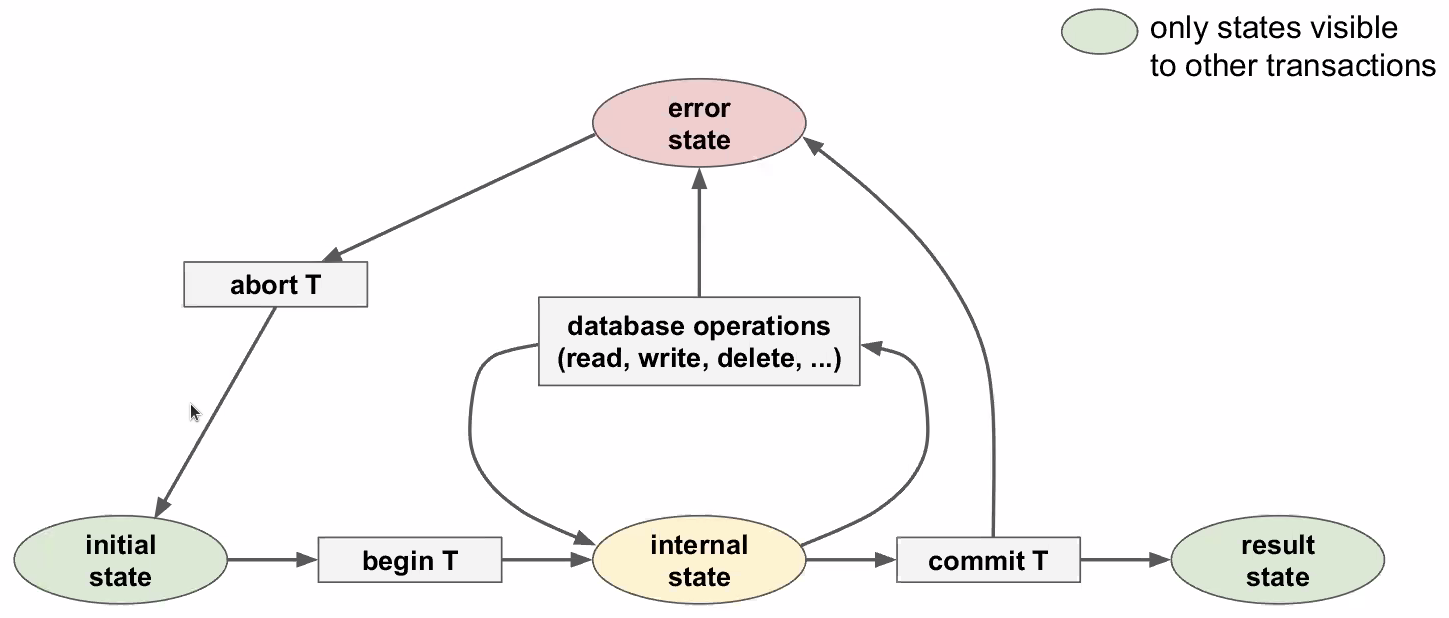
\includegraphics[width=0.9\linewidth]{cs2102-transition-graph.png}
  \end{tightcenter}

  \subsubsection{ACID properties}
  \begin{enumerate}
    \item \textbf{Atomicity} \(\rightarrow\) either all effects of $ T $ are reflected in the database, or none
    \item \textbf{Consistency}  \(\rightarrow\) the execution of $ T $ guarantees to yield a \textit{correct state} of the DB
    \item \textbf{Isolation} \(\rightarrow\)  execution of T is \textit{isolated} from the effects of concurrent transactions
    \item \textbf{Durability} \(\rightarrow\) after the commit of $ T $, its effects are \textit{permanent}  in case of failures
  \end{enumerate}

  \subsection{Serial vs Concurrent Execution}
  \begin{minipage}[t]{0.50\linewidth}
    \subsubsection{Serial Execution}
    \begin{itemize}
      \item $ \checkmark $ \textit{correct} final result
      \item $ \times $ less (unoptimised) resource utilisation; low throughput
    \end{itemize}
  \end{minipage}
  \ 
  \begin{minipage}[t]{0.48\linewidth}
    \subsubsection{Concurrent Execution}
    \begin{itemize}
      \item $\times$ potential issues: lost update / dirty read / unrepeatable read
    \end{itemize}
  \end{minipage}

  \subsubsection{Serializability}
  \begin{itemize}
    \item Requirement for Concurrent Execution: \textbf{serializable transaction execution} 
    \item (concurrent execution of a set of transactions is) \definition{serializable} execution is equivalent to some serial execution of the same set of transactions
      \begin{itemize}
        \item \definition{equivalent} \(\rightarrow\) they have the same \textit{effect}  on the data
      \end{itemize}
  \end{itemize}

  \subsubsection{Core tasks of DBMS}
  \begin{itemize}
    \item Support \textit{concurrent executions} of transactions - to optimise performance
    \item enforce \textit{serializability} of concurrent executions - to ensure integrity of data
  \end{itemize}

  \section{01-1. RELATIONAL MODEL}
  \begin{itemize}
    \item \definition{relation schema} defines a relation
      \begin{itemize}
        \item specifies the \textbf{attributes} (columns) and data constraints
        \item \definition{data constraints} limits the kind of data you can put into the database
      \end{itemize}
    \item \definition{relational database schema} set of relation schemas + data constraints
      \begin{itemize}
        \item TableName(col\_1, col\_2, col\_3) with dom(col\_1) = \{x, y, z\}, ...
      \end{itemize}
    \item \definition{relational database} collection of tables
  \end{itemize}

  \begin{itemize}
    \item \definition{domain} a set of \textit{atomic} values
      \begin{itemize}
        \item domain of attribute $ A_i $, $ dom(A_i) =$ set of possible values for $ A_i $
        \item for each value $ v $ of attribute $ A_i $, $ v \in dom(A_i) $ or $ v = $ \code{null}
          \begin{itemize}
            \item \code{null}: special value indicating that $ v $ is not known or specified
          \end{itemize}
        \item e.g. dom(course) = \{cs2102, cs2030, cs2040\}
      \end{itemize}
    \item \definition{relation} a set of \textit{tuples} 
      \begin{itemize}
        \item $ R(A_1, A_2, \dots, A_n) $ : relation schema with name $ R $ and $ n $ attributes $ A_1, A_2, \dots, A_n $
        \item each instance of schema $ R $ is a relation which is a subset of $ \{(a_1, a_2, \dots, a_n) \mid a_i \in dom(A_i) \cup \{null\}\} $
      \end{itemize}
  \end{itemize}


  \subsection{Data Integrity}
  \begin{itemize}
    \item \definition{integrity constraint} condition that restricts what constitutes valid data
      \begin{itemize}
        \item DBMS will check that tables only ever contain valid data
      \end{itemize}
    \item \definition{structural} (integrity) inherent to the data model 
    \item 3 main strucutral integrity constraints of the Relation Model
      \begin{enumerate}
        \item Domain constraints
        \item Key constraints
        \item Foreign key constraints
      \end{enumerate}
  \end{itemize}

  \subsection{Key Constraints}
  \begin{itemize}
    \item \definition{superkey} subset of attributes that \textit{uniquely} identifies a tuple in a relation
      \begin{itemize}
        \item e.g. \{id, title\}
      \end{itemize}
    \item \definition{key} superkey that is also \textbf{minimal} 
      \begin{itemize}
        \item no proper subset of the key is a superkey
        \item e.g. \{id\}
      \end{itemize}
    \item \definition{candidate keys} set of all keys for a relation
    \item \definition{primary key} selected candidate key for a relation
      \begin{itemize}
        \item \textit{cannot} be \code{null} $ \Rightarrow $  \textbf{entity integrity constraint} 
      \end{itemize}
  \end{itemize}

  \subsection{Foreign Key Constraints}
  \begin{itemize}
    \item \definition{foreign key} subset of attributes of relation $ A $ if it refers to the \textit{primary key}  in a relation $ B $.
    \item each foreign key in a relation must:
      \begin{enumerate}
        \item appear as a \textbf{primary key} in the referenced relation, OR:
        \item be a \code{null} value
      \end{enumerate}
  \end{itemize}

  \section{01-2. SUMMARY}
  \begin{tightcenter}
    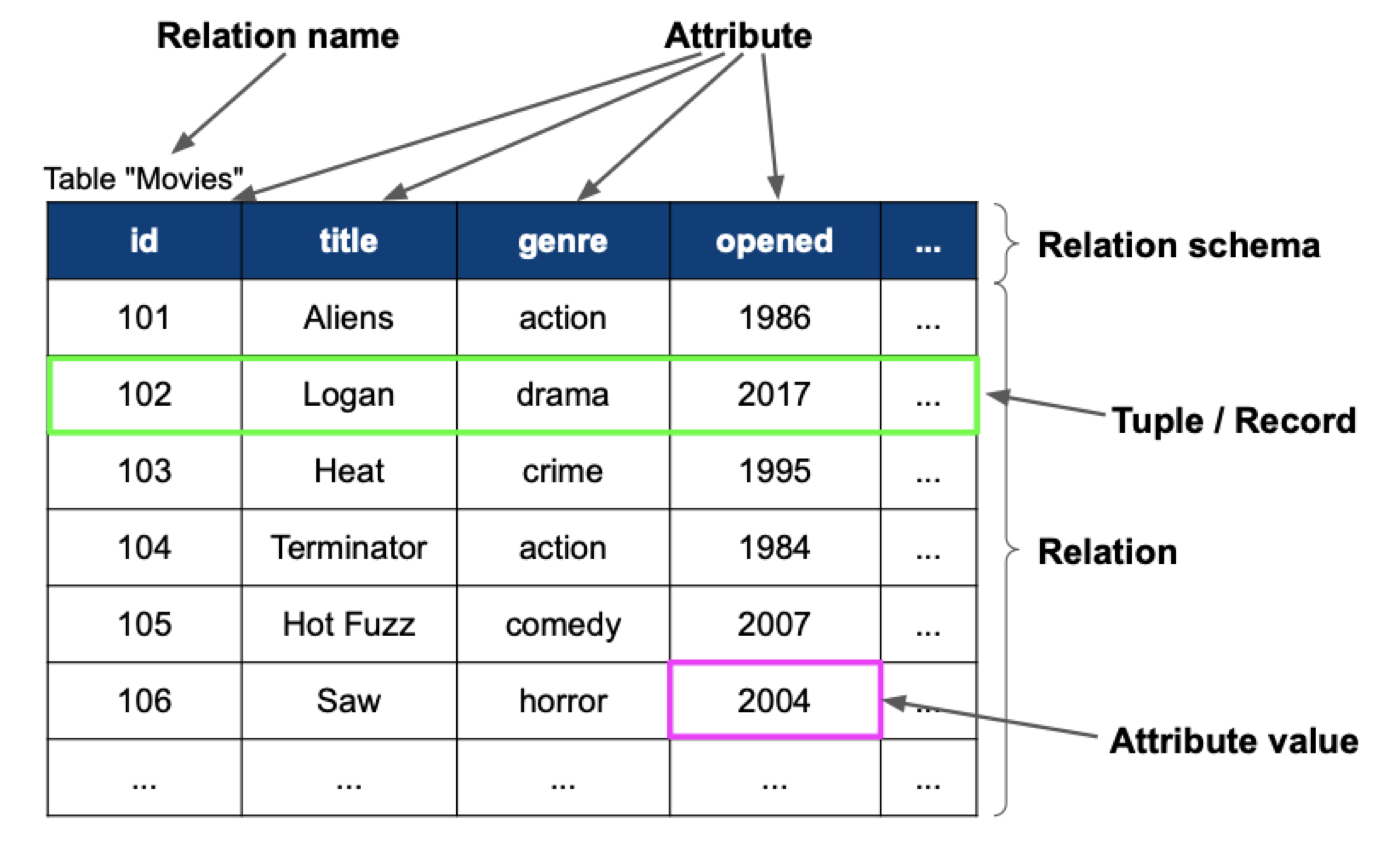
\includegraphics[width=0.9\linewidth]{cs2102-relational-model-example.png}
  \end{tightcenter}

  \section{02. RELATIONAL ALGEBRA}
  \begin{itemize}
    \item \definition{algebra} mathematical system of operands and operators
      \begin{itemize}
        \item \textbf{operands}: variables or values from which new values can be constructed
        \item \textbf{operators}: symbols denoting procedures that construct new values from given values
      \end{itemize}
    \item \definition{relation algebra} procedural query language
      \begin{itemize}
        \item \textbf{operands}: relations or variables representing relations
        \item \textbf{operators}: transform one or more input relations into one output relation
      \end{itemize}
  \end{itemize}

  \subsection{Closure Property}
  \begin{itemize}
    \item \definition{closure} relations are \textit{closed}  under relational algebra
      \begin{itemize}
        \item all input operands and outputs of all operators are \textit{relations} 
        \item the output of one operator can serve as input for subsequent operators
      \end{itemize}
    \item allows for nesting of relational operators $\Rightarrow$ \textbf{relational algebra expressions} 
  \end{itemize}

  \section{02-1. BASIC OPERATORS}
  \subsection{UNARY OPERATORS}

  \subsubsection{Selection, $ \sigma_c $}
  \begin{itemize}
    \item \definition{$\sigma_c(R)$} selects all tuples from a relation  $ R $ that satisfy condition $ c $.
      \begin{itemize}
        \item for each tuple $ t \in R$, $\; t \in \sigma_c(R) \iff c $ evaluates to true on $ t $ 
        \item input and output relation have the same schema
      \end{itemize}
    \item \definition{selection condition} 
      \begin{itemize}
        \item a \textit{boolean expression} of one of the following forms:
          \begin{itemize}
            \item constant selection - attribute \textbf{op} constant
            \item attribute selection - attribute$_1$ \textbf{op} attribute$_2$
            \item expr$_1 \land $ expr$ _2 ; \quad$ expr$_1 \lor $ expr$ _2 ; \quad$ item $ \lnot $ expr $ ; \quad $(expr)
          \end{itemize}
        \item with \textbf{op} $\in \{=, <>, <, \leq, \geq, >\}$
          \begin{itemize}
            \item \textbf{operator precedence}: (), \textbf{op}, $\lnot$, $\land$, $\lor$
          \end{itemize}
        \item handling \code{null} values
          \begin{itemize}
            \item comparison operation with \code{null} $\Rightarrow$ \textbf{unknown} 
            \item arithmetic operation with \code{null} $\Rightarrow$ \code{null} 
          \end{itemize}
      \end{itemize}
  \end{itemize}

  \subsubsection{Projection, $\pi_\ell$}
  \begin{itemize}
    \item \definition{$\pi_\ell(R)$} projects all attributes of a given \textbf{relation}  specified in list $\ell$
      \begin{itemize}
        \item \textit{relation} = set of tuples $\Rightarrow$ duplicates removed from output relation!
        \item \textbf{order} of attributes matters!
      \end{itemize}
  \end{itemize}

  \subsubsection{Renaming, $\rho_\ell$}
  \begin{itemize}
    \item \definition{$\rho_\ell(R)$} renames the attributes of a relation  $R$ (schema $R(A_1, A_2, \dots, A_n)$)
    \item 2 possible formats for $\ell$
      \begin{itemize}
        \item $\ell$ is the new \textit{schema} in terms of the new attribute names
          \begin{itemize}
            \item $\ell = (B_1, B_2, \dots, B_n)$; $B_i = A_i$ if attribute $A_i$ does not get renamed
          \end{itemize}
        \item $\ell$ is a list of attribute renamings of the form: $B_i \leftarrow A_i, \dots, B_k \leftarrow A_k$
          \begin{itemize}
            \item each renaming $B_j \leftarrow A_j$ renames attribute $A_j$ to attribute $B_j$
            \item order of renaming doesn't matter
          \end{itemize}
      \end{itemize}
  \end{itemize}

  \subsection{SET OPERATORS}
  \begin{itemize}
    \item \definition{union} $R \cup S$ returns a relation with all tuples in both $R$ \textbf{or}  $S$
    \item \definition{intersection} $R \cap S$ ... all tuples in both $R$ \textbf{and}  $S$ 
    \item \definition{set difference} $R - S$ ... all the tuples in  $R$ \textbf{but not in}  $S$
  \end{itemize}
  ! requirement for all set operators: $R$ and $S$ must be \textbf{union-compatible} 

  \subsubsection{Union Compatibility}
  \begin{itemize}
    \item two relations $R$ and $S$ are \definition{union-compatible} if
      \begin{itemize}
        \item $R$ and $S$ have the same number of attributes; and
        \item the corresponding attributes have the \textit{same or compatible domains} 
      \end{itemize}
    \item note: $R$ and $S$ do not have to use the same attribute names
  \end{itemize}

  \subsection{CROSS PRODUCT}
  \begin{itemize}
    \item \definition{cross product} given two relations $R(A, B, C)$ and $S(X, Y)$,  
      \\* $R \times S$ returns a relation with schema $(A, B, C, X, Y)$ defined as 
      \\* $R \times S = \{(a, b, c, x, y) \mid (a, b, c) \in R, (x, y) \in S\}$
      \begin{itemize}
        \item combines two relations $R$ and $S$ by forming all pairs of tuples from the relations
      \end{itemize}
    \item \textbf{size} of cross product $= \abs{R}*\abs{S}$
  \end{itemize}

  \section{02-2. JOIN OPERATORS}

  \subsection{Inner Joins} 
  \begin{itemize}
    \item eliminate all tuples that do not satisfy a matching criteria (i.e. \textbf{attribute selection} )
  \end{itemize}
  \subsubsection{$\theta$-join}
  \begin{itemize}
    \item \definition{$\theta$-join} (of two relations $R$ and $S$) \( {\displaystyle{R \bowtie_\theta S = \sigma_\theta(R \times S)}} \) 
  \end{itemize}

  \subsubsection{Equi Join $\Join$}
  \begin{itemize}
    \item special case of $\theta$-join defined over the  \textbf{equality} operator ($=$) only
  \end{itemize}

  \subsubsection{Natural Join $\Join$}
  \begin{itemize}
    \item the \definition{natural join} (of two relations $R$ and $S$) is defined as 
      \\* $R \Join S = \pi_\ell(R\Join_c \rho_{b_i \leftarrow a_i, \dots, b_k \leftarrow a_k}(S))$
      \begin{itemize}
        \item $A=\{a_i, \dots, a_k\}$ is the set of attributes that $R$ and $S$ have in common
        \item $c = ((a_i = b_i) \land \dots \land (a_k = b_k))$
        \item $\ell =$ list of all attributes of $R$ + list of all attributes in $S$ that are \textbf{not in}  $A$
      \end{itemize}
    \item performed over all attributes that $R$ and $S$ have in common
      \begin{itemize}
        \item no explicit matching criteria has to be specified
      \end{itemize}
    \item output relation contains the common attributes of $R$ and $S$ only \textit{once} 
  \end{itemize}

  \subsection{Outer Joins}
  \begin{itemize}
    \item \definition{dangling tuples} tuples in $R$ or $S$ that do not match with tuples in the other relation
      \begin{itemize}
        \item \definition{$\textit{dangle}(R \Join_\theta S)$} set of dangling tuples in  $R$ wrt to $R \Join_\theta S$
          \begin{itemize}
            \item $\textit{dangle}(R \Join_\theta S) \subseteq R$
          \end{itemize}
        \item always removed by inner joins, kept by outer joins
        \item missing attribute values are padded with \code{null} 
      \end{itemize}
    \item \definition{$null(R)$} $n$-component \textbf{tuple}  of \code{null} values where $n$ is the number of attributes of $R$
  \end{itemize}

  \subsubsection{Definitions}
  \begin{itemize}
    \item \definition{left outer join}$R \lojoin_\theta S = R \Join_\theta S \cup (\textit{dangle}(R \Join_\theta S) \times \{\textit{null}(S)\}) $
    \item \definition{right outer join}$R \rojoin_\theta S = R \Join_\theta S \cup (\{\textit{null}(R)\} \times \textit{dangle}(S \Join_\theta R))$
    \item \definition{full outer join}$R \fojoin_\theta S$
      \\* $= R \Join_\theta S \cup (\textit{dangle}(R \Join_\theta S) \times \{\textit{null}(S)\}) \cup (\{\textit{null}(R)\} \times \textit{dangle}(S \Join_\theta R))$
  \end{itemize}

  \subsubsection{Natural Outer Joins}
  \begin{itemize}
    \item natural left/right/full outer join: $R \lojoin S$ / $R \rojoin S$ / $R \fojoin S$
    \item only equality operator is used for the join condition
    \item join is performed over all attributes that R and S have in common
    \item output relation contains the common attributes of R and S only once
  \end{itemize}

  \section{03. SQL}
  \subsection{Overview}
  \begin{itemize}
    \item \textbf{domain-specific language} - used for relational databases
    \item \textbf{declarative language} - focuses on \textit{what} to compute, not \textit{how} to compute
    \item built on top of RA
    \item query = \code{SELECT} statement
  \end{itemize}

  \subsection{Data Types (psql)}
  \begin{itemize}
    \item user-defined types
    \item basic data types
      \begin{tightcenter}
        {\rowcolors{2}{gray!15}{gray!5}\begin{tabular}
            {ccc}
            \rowcolor{cyan!10} 
            \textbf{type} & \textbf{description} \\ \hline 
            boolean & logical Boolean \\ 
            integer & signed 4-byte integer \\
            float8 & double precision floating point number (8 bytes) \\
            numeric[(p, s)] & exact numeric of selectable preciison \\
            char(n) & fixed-length character string \\
            varchar(n) & variable-length character string \\
            text & variable-length character string \\
            date & calendar date (year month day) \\
            timestamp & date and time \\
            \hline
          \end{tabular}
        }
      \end{tightcenter}
    \item char, varchar, text: different sizes to optimise storage
      \begin{itemize}
        \item \code{varchar(n)} - $n$ is the maximum length 
        \item \code{char(n)} - storage size = maximum size = n (will be padded up to $n$ bytes)
        \item \code{text} - usually for very long strings
      \end{itemize}
  \end{itemize}

  \subsection{Types of Commands/Statements}
  \begin{tightcenter}
    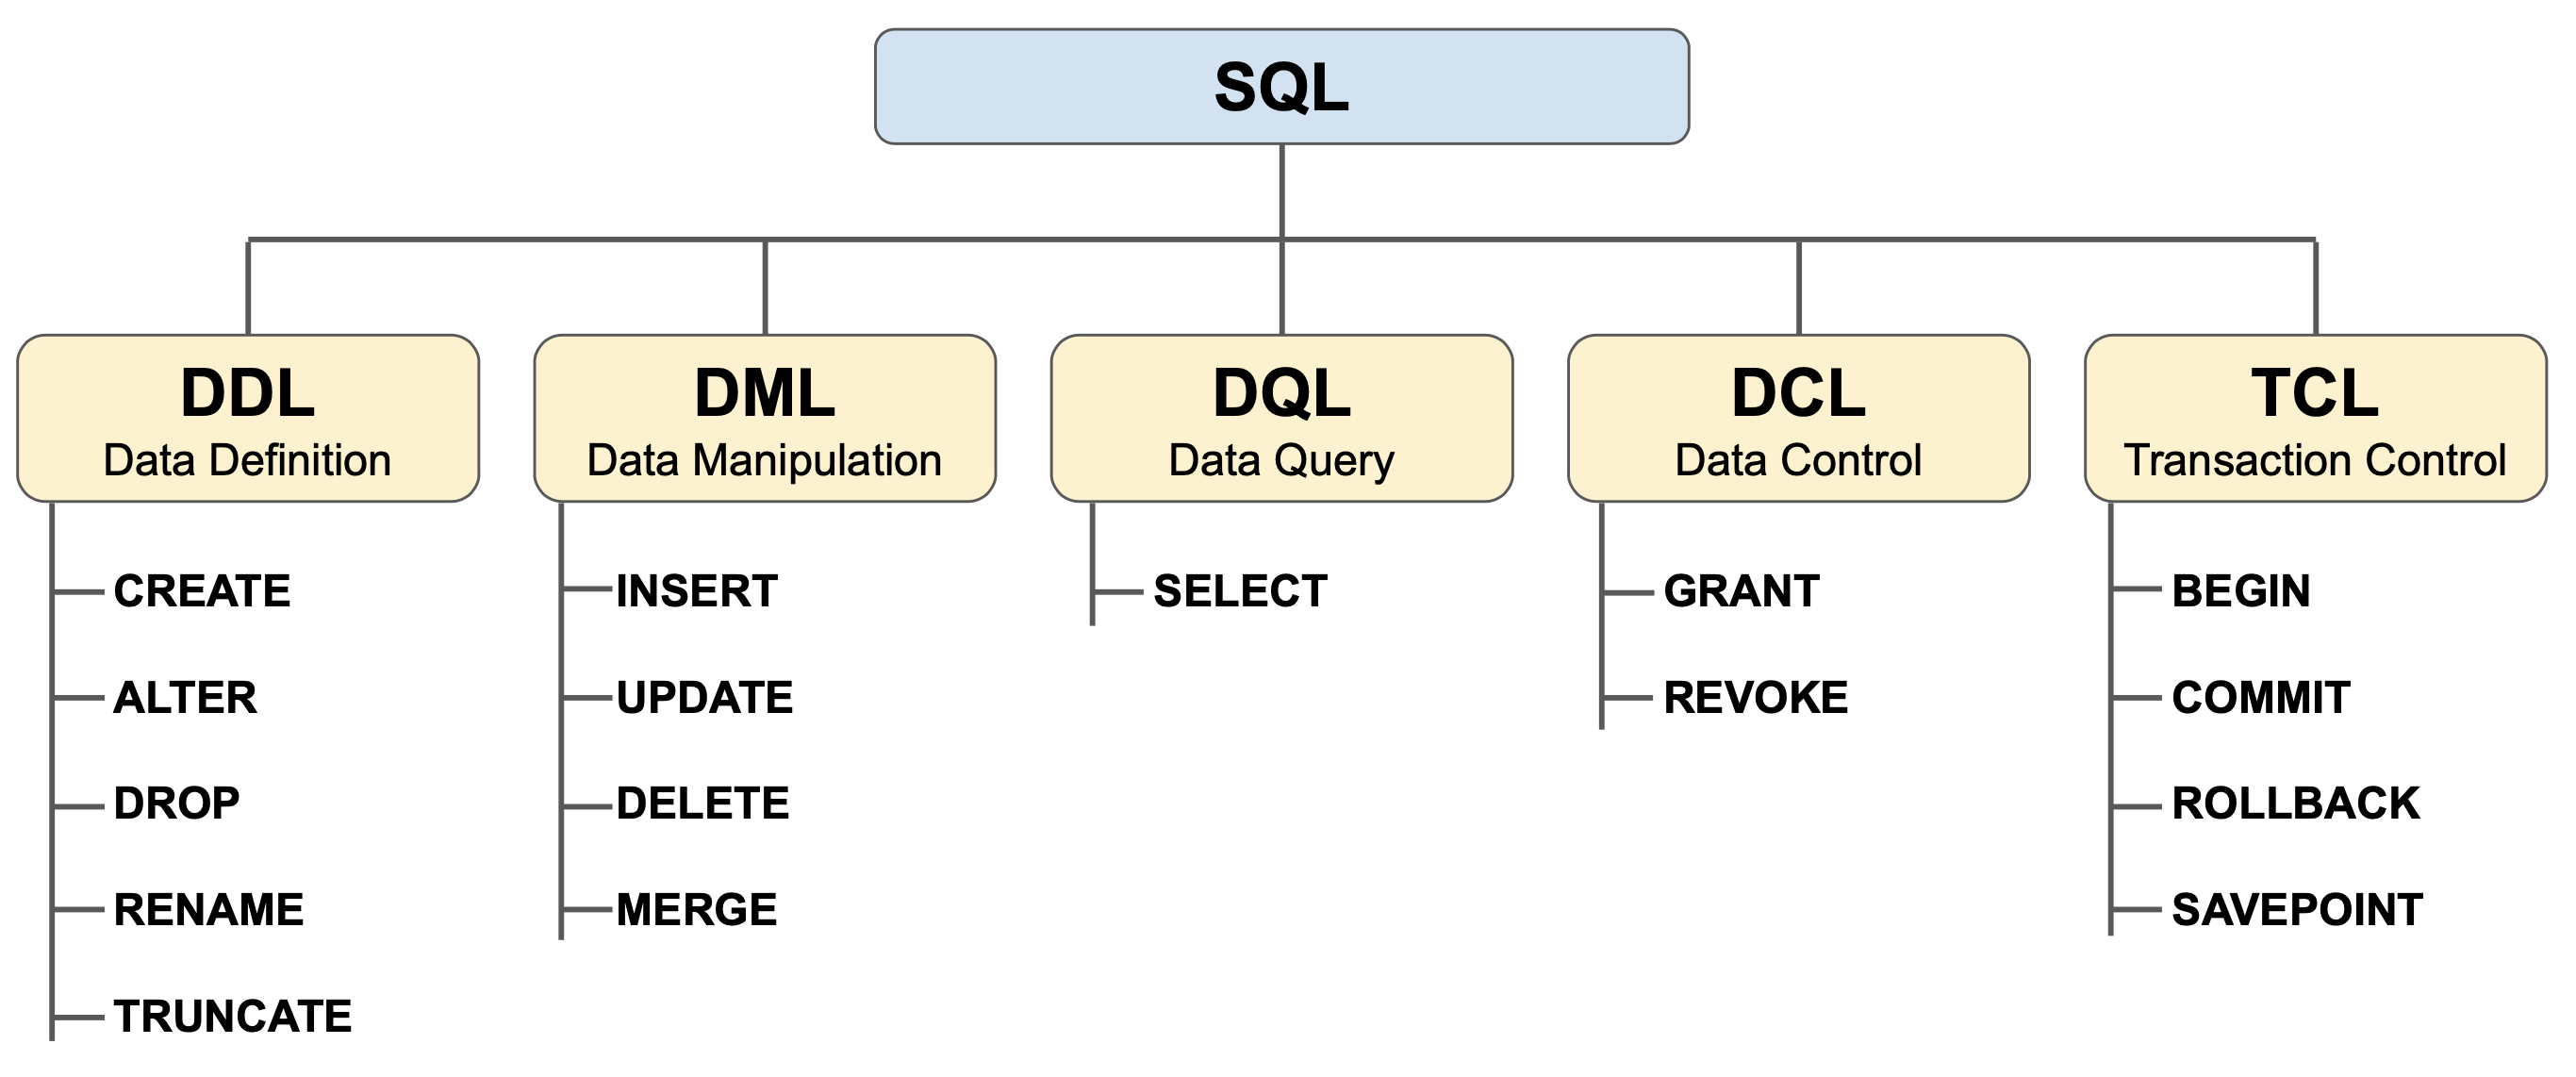
\includegraphics[width=0.9\linewidth]{cs2102-sql-query-types.png}
  \end{tightcenter}

  \subsection{DDL (Data Definition)}

  \subsubsection{Create Tables}
  \begin{lstlisting}[style=mySQL]
CREATE TABLE Employees (
  id     INTEGER,
  name   TEXT,
  role   VARCHAR(50)
);
  \end{lstlisting}

  \subsubsection{Insert Data}
  \begin{lstlisting}[style=mySQL]
-- specifying all attribute values
INSERT INTO Employees VALUES (101, 'John', 25, 'developer');
-- specifying selected attribute values
INSERT INTO Employees (id, name) VALUES (102, 'Smith');
  \end{lstlisting}

  \subsubsection{Modify Schema}
  \begin{lstlisting}[style=mySQL]
-- change data type 
ALTER TABLE Projects ALTER COLUMN name TYPE VARCHAR(200); 
-- set default value 
ALTER TABLE Projects ALTER COLUMN start_year SET DEFAULT 2021; 
-- drop default value
ALTER TABLE Projects ALTER COLUMN start_year DROP DEFAULT; 
-- add new column with a default value
ALTER TABLE Projects ADD COLUMN budget NUMERIC DEFAULT 0.0; 
-- drop column from table
ALTER TABLE Projects DROP COLUMN budget; 
-- add constraint
ALTER TABLE Teams ADD CONSTRAINT eid_fkey FOREIGN KEY (eid) REFERENCES Employees (id);
-- drop constraint
ALTER TABLE Teams DROP CONSTRAINT eid_fkey; /* eid_fkey = name of constraint */
  \end{lstlisting}

  \subsubsection{Drop Tables}
  \begin{lstlisting}[style=mySQL]
DROP TABLE Projects;
-- check first if table exists; avoids throwing an error
DROP TABLE IF EXISTS Projects; 
-- will also delete FK constraint (but not referencing tables)
DROP TABLE Projects CASCADE; 
  \end{lstlisting}

  \subsection{DML (Data Manipulation)}

  \subsubsection{Delete Data}
  \begin{lstlisting}[style=mySQL]
-- deletes all tuples 
DELETE FROM Employees; 
-- deletes selected tuples
DELETE FROM Employees WHERE role='developer';
  \end{lstlisting}

  \subsubsection{Update Data}
  \begin{lstlisting}[style=mySQL]
UPDATE Employees 
SET age = age + 1
WHERE name = 'John';

-- updates all values 
UPDATE Employees
SET name=UPPER(name), 
    job=UPPER(job);

-- updates all values 
UPDATE Employees 
SET age = 0; 
  \end{lstlisting}

  \subsection{Handling NULLs}
  \begin{itemize}
    \item prerequisite for integrity constraints
    \item \textbf{comparison} operation with \code{null} $\Rightarrow$ \textit{unknown}
    \item \textbf{arithmetic} operation with \code{null} $\Rightarrow$ \code{null}
  \end{itemize}

  \subsubsection{IS (NOT) NULL comparison predicate}
  \begin{itemize}
    \item checks if values are equal to \code{null} 
      \begin{itemize}
        \item evaluates to true $\iff$ x is \code{null}
      \end{itemize}
    \item \code{x IS NOT NULL} $\equiv$ \code{NOT (x IS NULL)}
  \end{itemize}

  \subsubsection{IS (NOT) NOT DISTINCT comparison predicate}
  \begin{itemize}
    \item equivalent to $x <> y$ if $x$ and $ y$ are non-\code{null} values
      \begin{itemize}
        \item $x$ and $y$ both \code{null} $\Rightarrow$ \textit{false}
        \item only one value is \code{null} $\Rightarrow$ \textit{true}
      \end{itemize}
    \item \code{x IS NOT DISTINCT FROM y} $\equiv$ \code{NOT (x IS DISTINCT FROM y)}
  \end{itemize}
  \begin{tightcenter}
    {\rowcolors{2}{gray!15}{gray!5}\begin{tabular}
        {cccc}
        \rowcolor{cyan!10} 
        \textbf{x} & \textbf{y} & x<>y & \texttt{x IS DISTINCT FROM y} \\ \hline 
        1 & 1 & FALSE & FALSE \\ 
        1 & 2 & TRUE & TRUE \\
        \textit{null} & 1 & \textit{null} & TRUE \\
        \textit{null} & \textit{null} & \textit{null} & FALSE \\
        \hline
      \end{tabular}
    }
  \end{tightcenter}

  \section{03-1. CONSTRAINTS}
  \begin{itemize}
    \item \textbf{unnamed}: name assigned by DBMS
    \item \textbf{named}: name is specified - easier bookkeeping
    \item all column constraints can be specified as table constraints, except \code{NOT NULL}
      \begin{itemize}
        \item table constraints referring to a single column can be writen as column constraints
        \item column and table constraints can be combined
          \begin{lstlisting}[style=mySQL]
  ... id INTEGER NOT NULL,
  ...
  UNIQUE(id)
          \end{lstlisting}
      \end{itemize}
  \end{itemize}
  \subsection{Not-Null Constraints}
  \begin{itemize}
    \item \textbf{violation}: $\exists t \in$ Employees where \code{t.id IS NOT NULL} evaluates to \textbf{false}
      \begin{lstlisting}[style=mySQL]
CREATE TABLE Employees (
  id   INTEGER NOT NULL, /* unnamed */
  name VARCHAR(50) CONSTRAINT nn_name NOT NULL, /* named */
  age  INTEGER,
  job  VARCHAR(50),
);
      \end{lstlisting}
  \end{itemize}

  \subsection{Unique Constraints}
  \begin{itemize}
    \item \textbf{violation} (of a unique constraint defined on attributes $A$ and $B$):
      \begin{itemize}
        \item For any two tuples $t_i, t_k \in$ R, \\*
          $(t_i\cdot A <> t_k\cdot A)$ or  $(t_i\cdot B <> t_k \cdot B)$ evaluates to  \textbf{false}
        \item  !!! \code{null} rows will NOT violate unique key constraints
      \end{itemize}
      \begin{lstlisting}[style=mySQL]
-- column constraint
CREATE TABLE Employees (
  id   INTEGER UNIQUE, /* unnamed */
  pid  INTEGER CONSTRAINT u_id UNIQUE, /* named */
  name VARCHAR(50), age INTEGER,
  role VARCHAR(50)
);
      \end{lstlisting}
      \begin{lstlisting}[style=mySQL]
-- table constraint
CREATE TABLE Employees (
  id   INTEGER,
  name VARCHAR(50), 
  UNIQUE(id),  /* unnamed */,
  CONTRAINT u_name UNIQUE (name) /* named */
);
      \end{lstlisting}
    \item unique constraints for \textbf{multiple attributes} can only be specified using \textbf{table} constraints
      \begin{lstlisting}[style=mySQL]
CREATE TABLE Employees (
  id     INTEGER,
  name   VARCHAR(50),
  UNIQUE (id, name), /* unnamed */
  CONSTRAINT u_allocation UNIQUE (id, name)  /* named */
)
      \end{lstlisting}
  \end{itemize}

  \subsection{Primary Key Constraints}
  \begin{itemize}
    \item \definition{prime attributes} attributes of the primary key 
      \begin{itemize}
        \item cannot be null
      \end{itemize}
    \item primary key vs \code{UNIQUE NOT NULL}
      \begin{itemize}
        \item \code{UNIQUE NOT NULL} is a candidate key
        \item max 1 primary key, but any number of \code{UNIQUE NOT NULL} constraints
        \item FK constraints are only applicable to PKs in referenced table
      \end{itemize}
      \begin{lstlisting}[style=mySQL]
-- PK constraint for one attribute
CREATE TABLE Teams (
  eid INTEGER PRIMARY KEY, 
  ... 
);
      \end{lstlisting}
      \begin{lstlisting}[style=mySQL]
-- PK constraint for multiple attributes
CREATE TABLE Teams (
  eid INTEGER,
  pname VARCHAR(100),
  PRIMARY KEY (ename, pname), /* unnamed */
  CONSTRAINT pk_alloc PRIMARY KEY (eid, pname) /* named */
);
      \end{lstlisting}
  \end{itemize}

  \subsection{Foreign Key Constraints}
  \begin{itemize}
    \item each FK in the referencing relation \textbf{must}:
      \begin{itemize}
        \item appear as a PK in the referenced relation, OR
        \item be a \code{null} value
      \end{itemize}
    \item referenced columns must be a PK or declared to be \textbf{unique}
    \item \texttt{R.sid} $\rightarrow$ \texttt{S.id}: \texttt{R.sid} is a FK referencing PK \texttt{id} in S
  \end{itemize}
  \begin{lstlisting}[style=mySQL]
CREATE TABLE Teams (
  eid INTEGER,
  pname VARCHAR(100),
  hours INTEGER,
  PRIMARY KEY (ename, pname),
  /* Teams.eid -> Employees.id */
  FOREIGN KEY (eid) REFERENCES Employees (id), 
  /* Teams.pname -> Projects.name */
  FOREIGN KEY (pname) REFERENCES Projects (name)
);
  \end{lstlisting}

  \subsubsection{specifications for table changes}
  \begin{itemize}
    \item \code{ON DELETE/UPDATE}: Specify action in case of the violation of a foreign key constraint
      \begin{itemize}
        \item attempting to delete primary key will throw error if ON DELETE not specified
        \item specify behavior when data in referenced table changes
      \end{itemize}
    \item possible actions:
      \begin{itemize}
        \item \code{NO ACTION}: (\textbf{default value}) - rejects the delete/update if it violates constraint
          \begin{itemize}
            \item \code{ON DELETE NO ACTION} - will raise error if key is referenced elsewhere
          \end{itemize}
        \item \code{RESTRICT}: similar to \code{NO ACTION}; checks that constraint cannot be deferred
        \item \code{CASCADE}: propagates delete/update to referencing tuples
        \item \code{SET DEFAULT}: updates FKs of referencing tuples to a specified default value
          \begin{itemize}
            \item !! default value must be a PK in the referenced table !!
            \item e.g. \code{... pid INTEGER DEFAULT 1, ...}
          \end{itemize}
        \item \code{SET NULL}: update FKs of referencing tuples to \code{null}
          \begin{itemize}
            \item be careful for primary attributes
            \item corresponding column must be allowed to contain \code{null} values!
          \end{itemize}
      \end{itemize}
  \end{itemize}
  \begin{lstlisting}[style=mySQL]
CREATE TABLE Teams (
  eid INTEGER,
  pname VARCHAR(100),
  hours INTEGER,
  PRIMARY KEY (ename, pname),
  FOREIGN KEY (eid) REFERENCES Employees (id) ON DELETE <action> ON UPDATE <action>,
  FOREIGN KEY (pname) REFERENCES Projects (name) ON DELETE NO ACTION ON UPDATE CASCADE 
  /* 'NO ACTION' is optional since it's default */
);
  \end{lstlisting}

  \subsection{Check Constraint}
  \begin{itemize}
    \item specify that column values must satisfy a boolean expression
    \item scope: one table, single row
    \item not a structural integrity constraint
      \begin{lstlisting}[style=mySQL]
-- column constraint
CREATE TABLE Teams (
  eid INTEGER,
  hours INTEGER check (hours > 0), /* unnamed */
  minutes INTEGER constraint positive_hours check (hours > 0) /* named */
);  
      \end{lstlisting}
      \begin{lstlisting}[style=mySQL]
-- table constraint
CREATE TABLE Teams (
  eid INTEGER,
  ...
  CHECK (hours <= end_year), /* unnamed table */
  CONSTRAINT valid_lifetime CHECK (start_year <= end_year) /* named table */
);  
      \end{lstlisting}
    \item \code{CHECK} constraints can be complex boolean expressions:
      \begin{lstlisting}[style=mySQL]
CREATE TABLE Teams (
  ...
  CHECK (
    (pname = 'Hello' AND hours >= 30)
    OR
    (panme <> 'Hello' AND hours > 0)
  )
);  
      \end{lstlisting}
  \end{itemize}

  \subsection{Deferrable Constraints}
  \begin{itemize}
    \item default behaviour for constraints: checked immediately at the end of SQL statement execution
      \begin{itemize}
        \item violation causes statement to be rolled back
      \end{itemize}
    \item \textbf{deferrable constraints}: relaxed constraint checks
      \begin{itemize}
        \item check will be deferred to the \textit{end} of the transaction
        \item available for: \code{UNIQUE}, \code{PRIMARY KEY}, \code{FOREIGN KEY}
      \end{itemize}
    \item advantages
      \begin{itemize}
        \item no need to care about order of SQL statements within a transaction
        \item allows for cyclic FK constraints
        \item performance boost (when constraint checks are bottleneck)
      \end{itemize}
    \item disadvantages
      \begin{itemize}
        \item harder to troubleshoot
        \item data definition is no longer unambiguous
        \item performance penalty when performing queries
      \end{itemize}
  \end{itemize}
  \subsubsection{syntax}
  \begin{itemize}
    \item \code{NOT DEFERRABLE} - (\textbf{default}) immediate check of constraint, cannot be changed 
    \item \code{DEFERRABLE INITIALLY IMMEDIATE} - immediate check of constraint by default, but can be changed
    \item \code{DEFERRABLE INITIALLY DEFERRED} - deferred check of constraint by default, but can be changed
  \end{itemize}
  \begin{lstlisting}[style=mySQL]
CREATE TABLE Employees (
  id INTEGER PRIMARY KEY,
  name VARCHAR(50),
  manager INTEGER,
  CONSTRAINT manager_fkey FOREIGN KEY (manager) REFERENCES Employees (id) DEFERRABLE INITIALLY IMMEDIATE 
);

BEGIN;
SET CONSTRAINT manager_fkey DEFERRED; 
  -- set check of constraint from "immediate" to "deferred"
DELETE FROM Employees WHERE id = 102; 
  -- constraint violated but not checked
UPDATE Employees SET manager = 101 WHERE id = 103; 
  -- constraint re-established
COMMIT;
  \end{lstlisting}

  \section{04. ENTITY RELATIONSHIP MODEL}
  \begin{itemize}
    \item all data is described in terms of \textbf{entities} and their \textbf{relationships}
    \item \definition{entity} objects that are distinguishable from other objects
      \begin{itemize}
        \item \definition{entity set} collection of entities of the same type
      \end{itemize}
    \item \definition{attribute} specific information describing an entity
      \begin{itemize}
        \item \definition{key attribute} uniquely identifies each entity (underline)
        \item \definition{composite attribute} composed of multiple other attributes (oval of ovals)
        \item \definition{multivalued attribute} may comprise more than one value for a given entity (double-lined oval)
        \item \definition{derived attribute} derived from other attributes (dashed oval)
      \end{itemize}
    \item \definition{relationship} association among two or more entities
      \begin{itemize}
        \item \definition{relationship set} collection of relationships of the same type
          \begin{itemize}
            \item may have their own attributes that describe the relationship
          \end{itemize}
      \end{itemize}
  \end{itemize}
  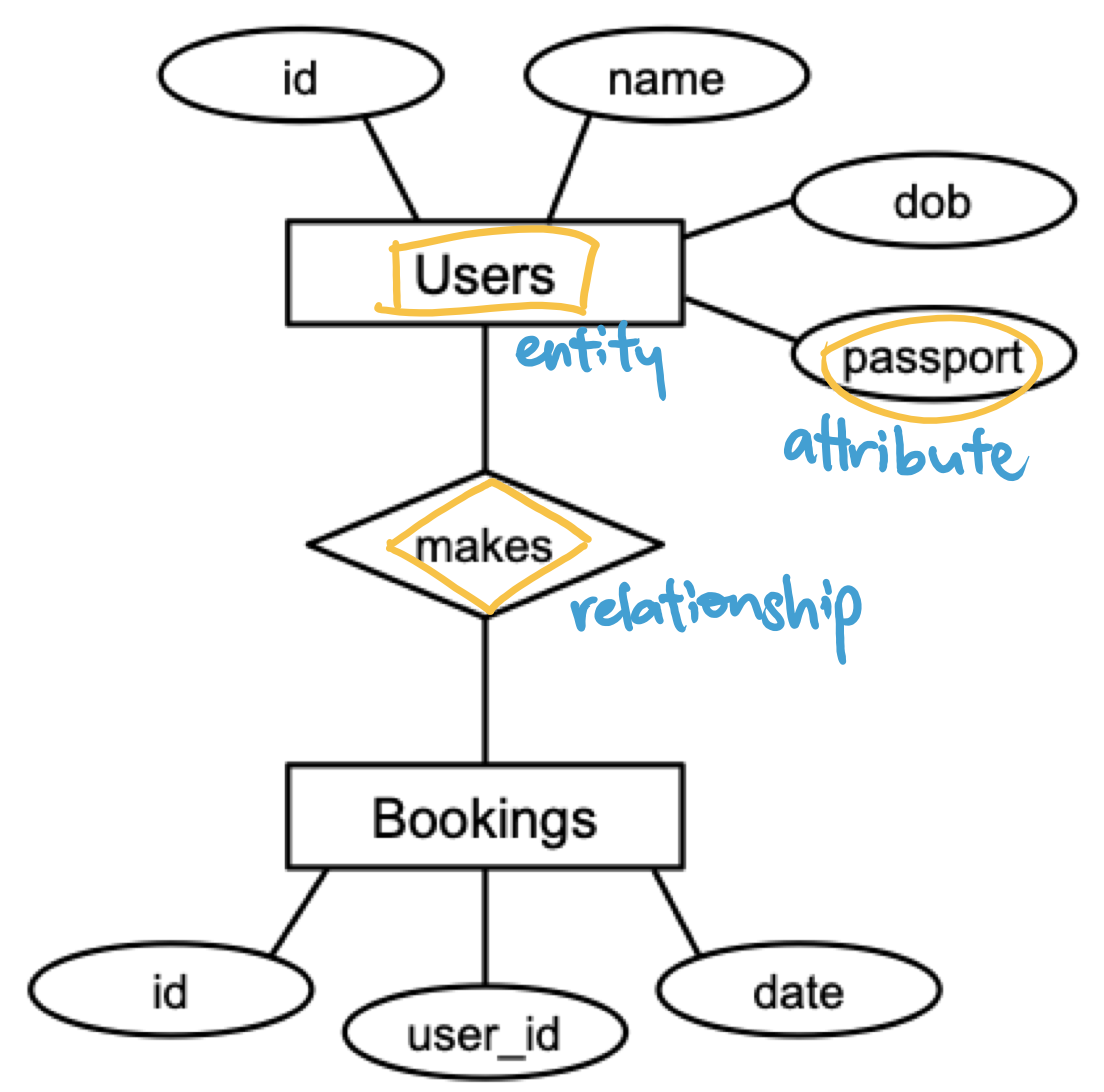
\includegraphics[width=0.4\linewidth]{cs2102-entity-relationship-model.png} 
  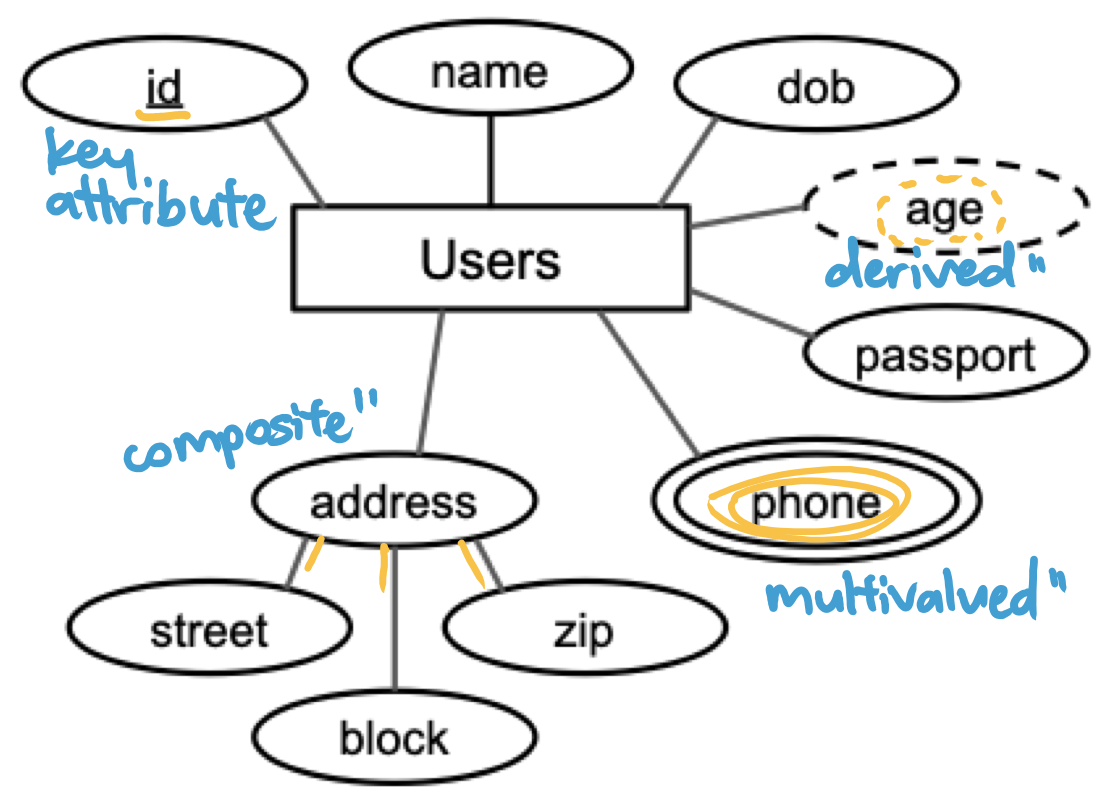
\includegraphics[width=0.5\linewidth]{cs2102-attribute-subtypes.png} 

  \subsubsection{relationship sets}
  \begin{itemize}
    \item \definition{role} descriptor of an entity set's participation in a relationship
      \begin{itemize}
        \item explicit role labels
      \end{itemize}
    \item \definition{degree} number of entity roles participating in a relationship 
      \begin{itemize}
        \item an $n$-ary relationship set involves $n$ entity roles (where $n$ is the degree of the relationship set)
        \item binary/ternary relationship set
        \item general $n$-ary relation:
          \begin{itemize}
            \item $n$ participating entity sets $E_1, E_2, \dots, E_n$ 
            \item $k$ relationship attributes $A_1, A_2, \dots, A_k$
            \item $Key(E_i)$  $\rightarrow$ the attributes of the selected key of entity set $E_i$
          \end{itemize}
      \end{itemize}
  \end{itemize}
  \begin{minipage}[c]{0.6\linewidth}
    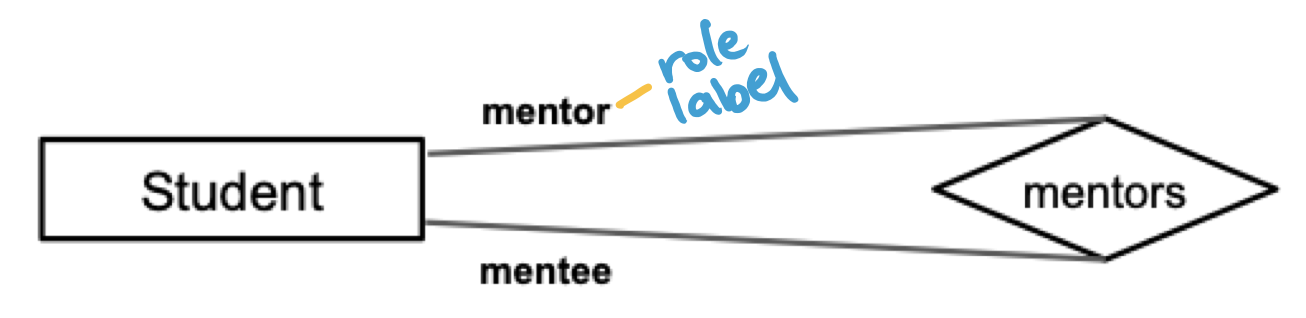
\includegraphics[width=0.95\linewidth]{cs2102-relationship-role-label.png} 
  \end{minipage}
  \begin{minipage}[c]{0.35\linewidth}
    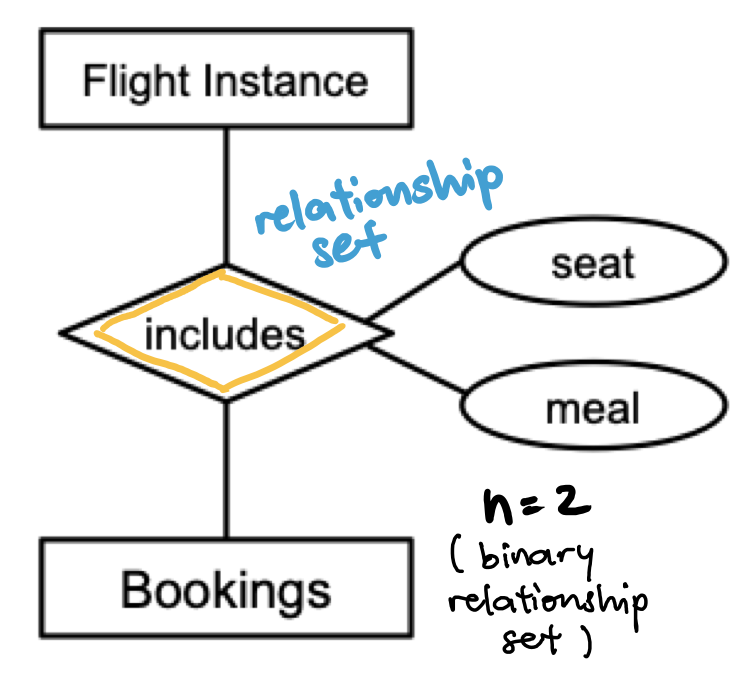
\includegraphics[width=0.95\linewidth]{cs2102-relationship-set.png} 
  \end{minipage}


  \subsection{Cardinality Constraints}
  \begin{itemize}
    \item describes how often an entity can participate in a relationship \textbf{at most}
    \item 3 basic cardinality constraints:
      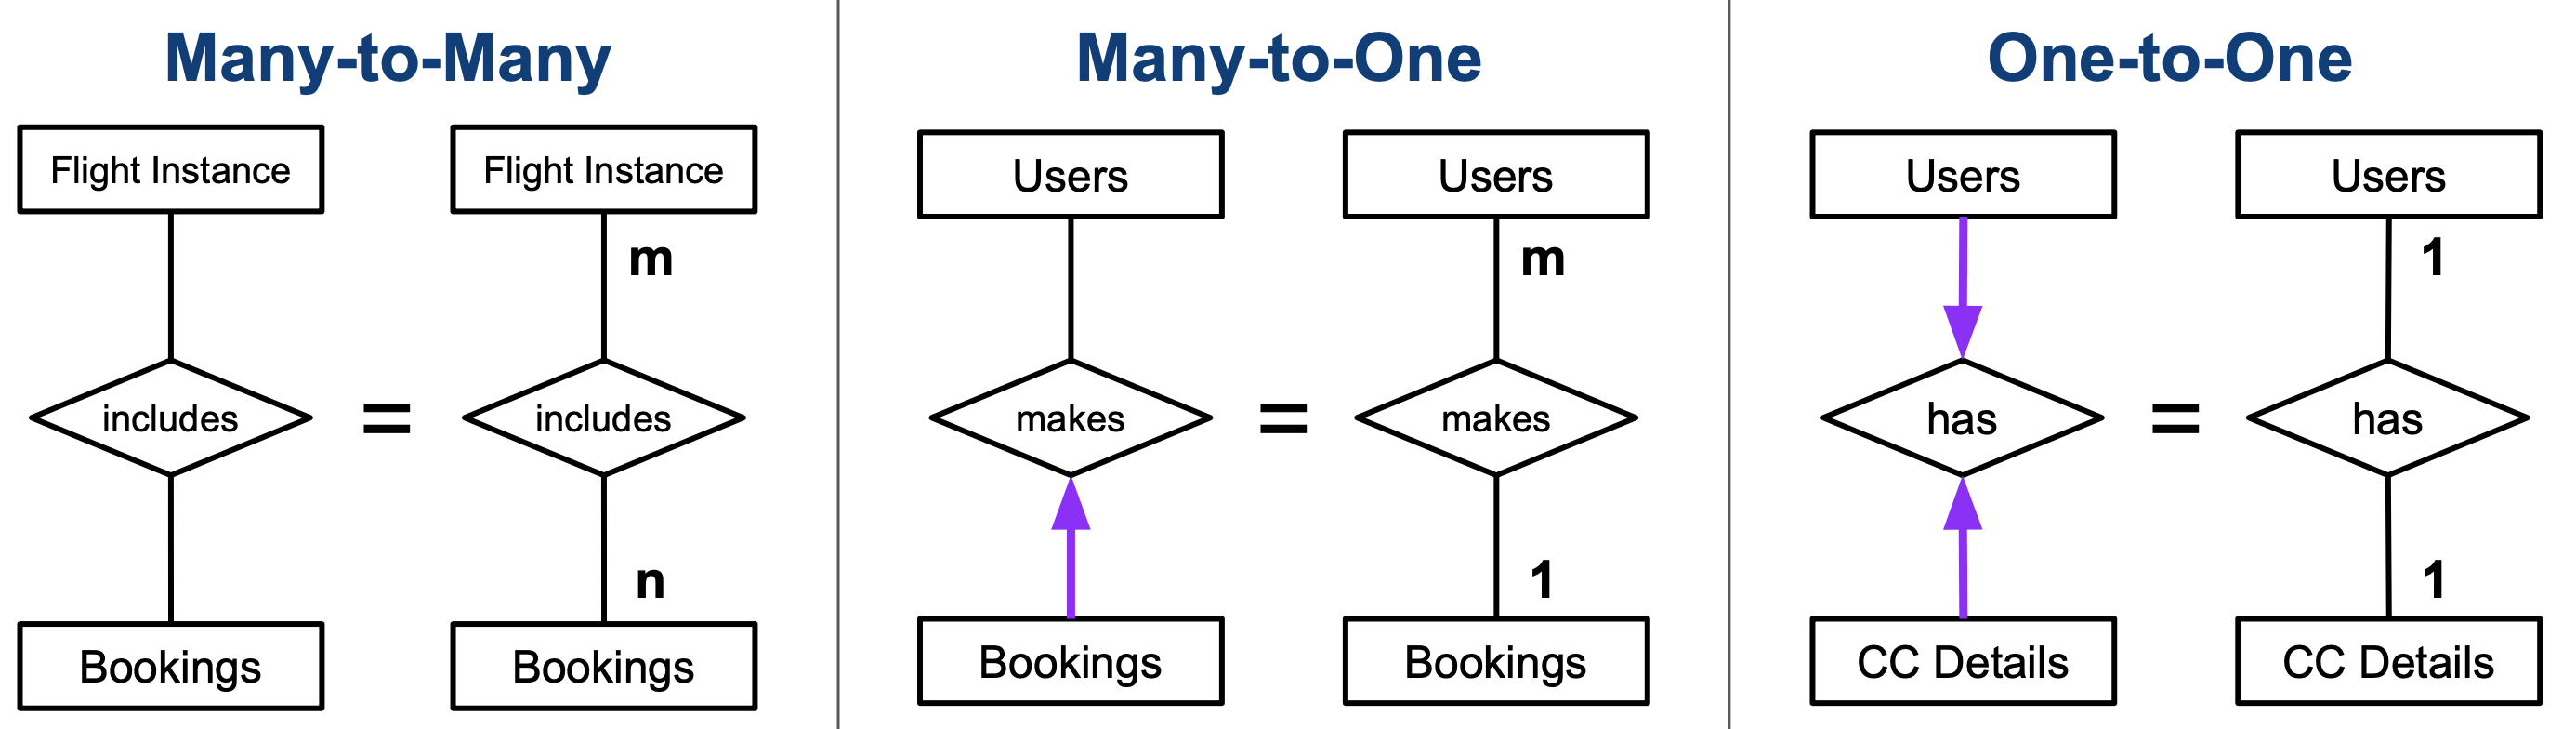
\includegraphics[width=0.95\linewidth]{cs2102-alternative-representation-cardinality-constraint.png} 
  \end{itemize}

  \subsection{Participation Constraints}
  \begin{itemize}
    \item specifies if an entity has to participate in a relationship (lower bound)
    \item \definition{partial participation constraint} participation (of an entity in a relationship) is not mandatory (0 or more)
    \item \definition{total participation constraint} participation is mandatory (1 or more)
  \end{itemize}
  \begin{center}
    \begin{multicols}{2}
      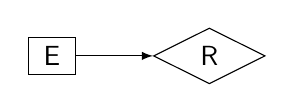
\begin{tikzpicture}
        \node[rectangle, draw, minimum width = 0.6cm] (e) at (0,0) {E};
        \node[diamond, draw, aspect = 2] (r) at (2,0) {R};
        \draw[-latex] (e) -- (r);
      \end{tikzpicture}
      \\* each instance of E participates in 
      \\* \textbf{at most one} instance of R
      \\ \ 

      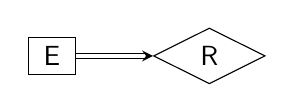
\begin{tikzpicture}
        \node[rectangle, draw, minimum width = 0.6cm] (e) at (0,0) {E};
        \node[diamond, draw, aspect = 2] (r) at (2,0) {R};
        \draw[-stealth, double, double distance = 1.2pt] (e) -- (r);
      \end{tikzpicture}
      \\* each instance of E participates in 
      \\* \textbf{exactly one} instance of R

      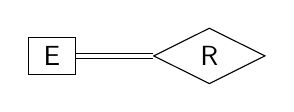
\begin{tikzpicture}
        \node[rectangle, draw, minimum width = 0.6cm] (e) at (0,0) {E};
        \node[diamond, draw, aspect = 2] (r) at (2,0) {R};
        \draw[double, double distance=1.2pt] (e) -- (r);
      \end{tikzpicture}
      \\* each instance of E participates in 
      \\* \textbf{at least one} instance of R
      \\ \ 

      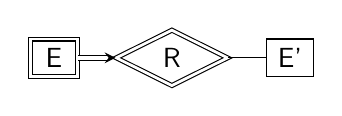
\begin{tikzpicture}
        \node[rectangle, double, draw, minimum width = 0.6cm, double distance=1pt] (e) at (0,0) {E};
        \node[diamond, double, draw, aspect = 2, double distance=1pt] (r) at (1.5,0) {R};
        \node[rectangle, draw, minimum width = 0.6cm] (e2) at (3,0) {E'};
        \draw[-stealth, double, double distance=1.2pt] (e) -- (r);
        \draw[-] (r) -- (e2);
      \end{tikzpicture}
      \\* E is a \textbf{weak entity set} 
      with identifying owner E' 
      \& identifying relationship set R.
    \end{multicols}
  \end{center}

  \subsection{Dependency Constraints}
  \begin{itemize}
    \item \definition{weak entity sets} entity set that does not have its own key 
      \begin{itemize}
        \item can only be uniquely identified through the primary key of its \textbf{owner entity}
        \item existence depends on the existence of its owner entity
        \item \definition{partial key} set of attributes of a weak entity set that uniquely identifies a weak entity for a given owner entity
          \begin{itemize}
            \item identifies the exact instance of a weak entity
              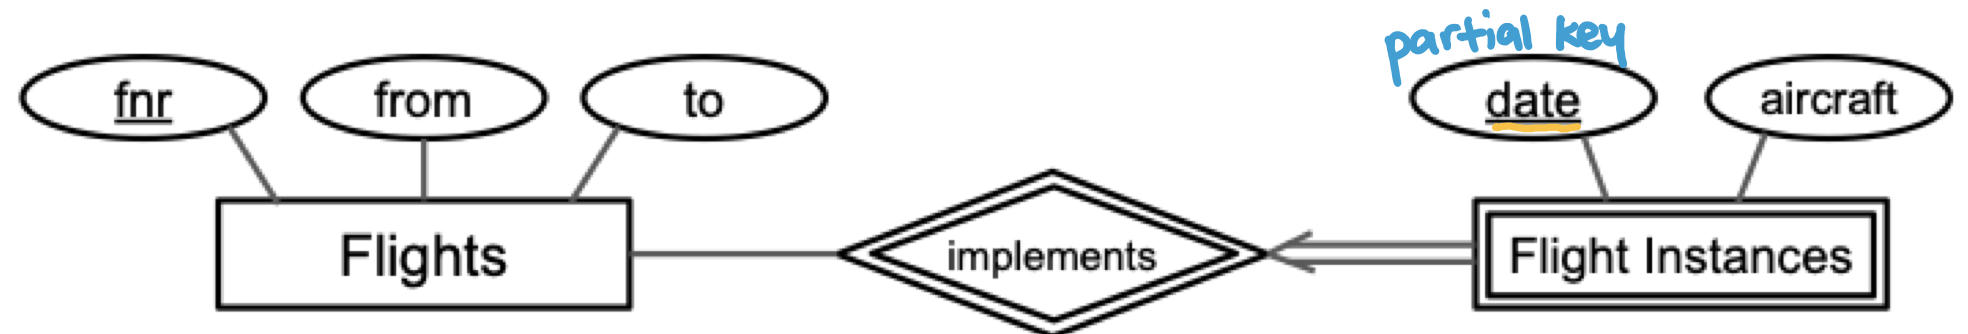
\includegraphics[width=0.85\linewidth]{cs2102-weak-entity-partial-key.png} 
          \end{itemize}
      \end{itemize}
    \item requirements
      \begin{enumerate}
        \item many-to-one relationship (identifying relationship) from weak entity set to owner entity set
        \item weak entity set must have \textbf{total participation} in identifying relationship
      \end{enumerate}
  \end{itemize}

  \subsection{Alternative Representations}
  \begin{tightcenter}
    \textbf{Min/Max notation}
    \\* 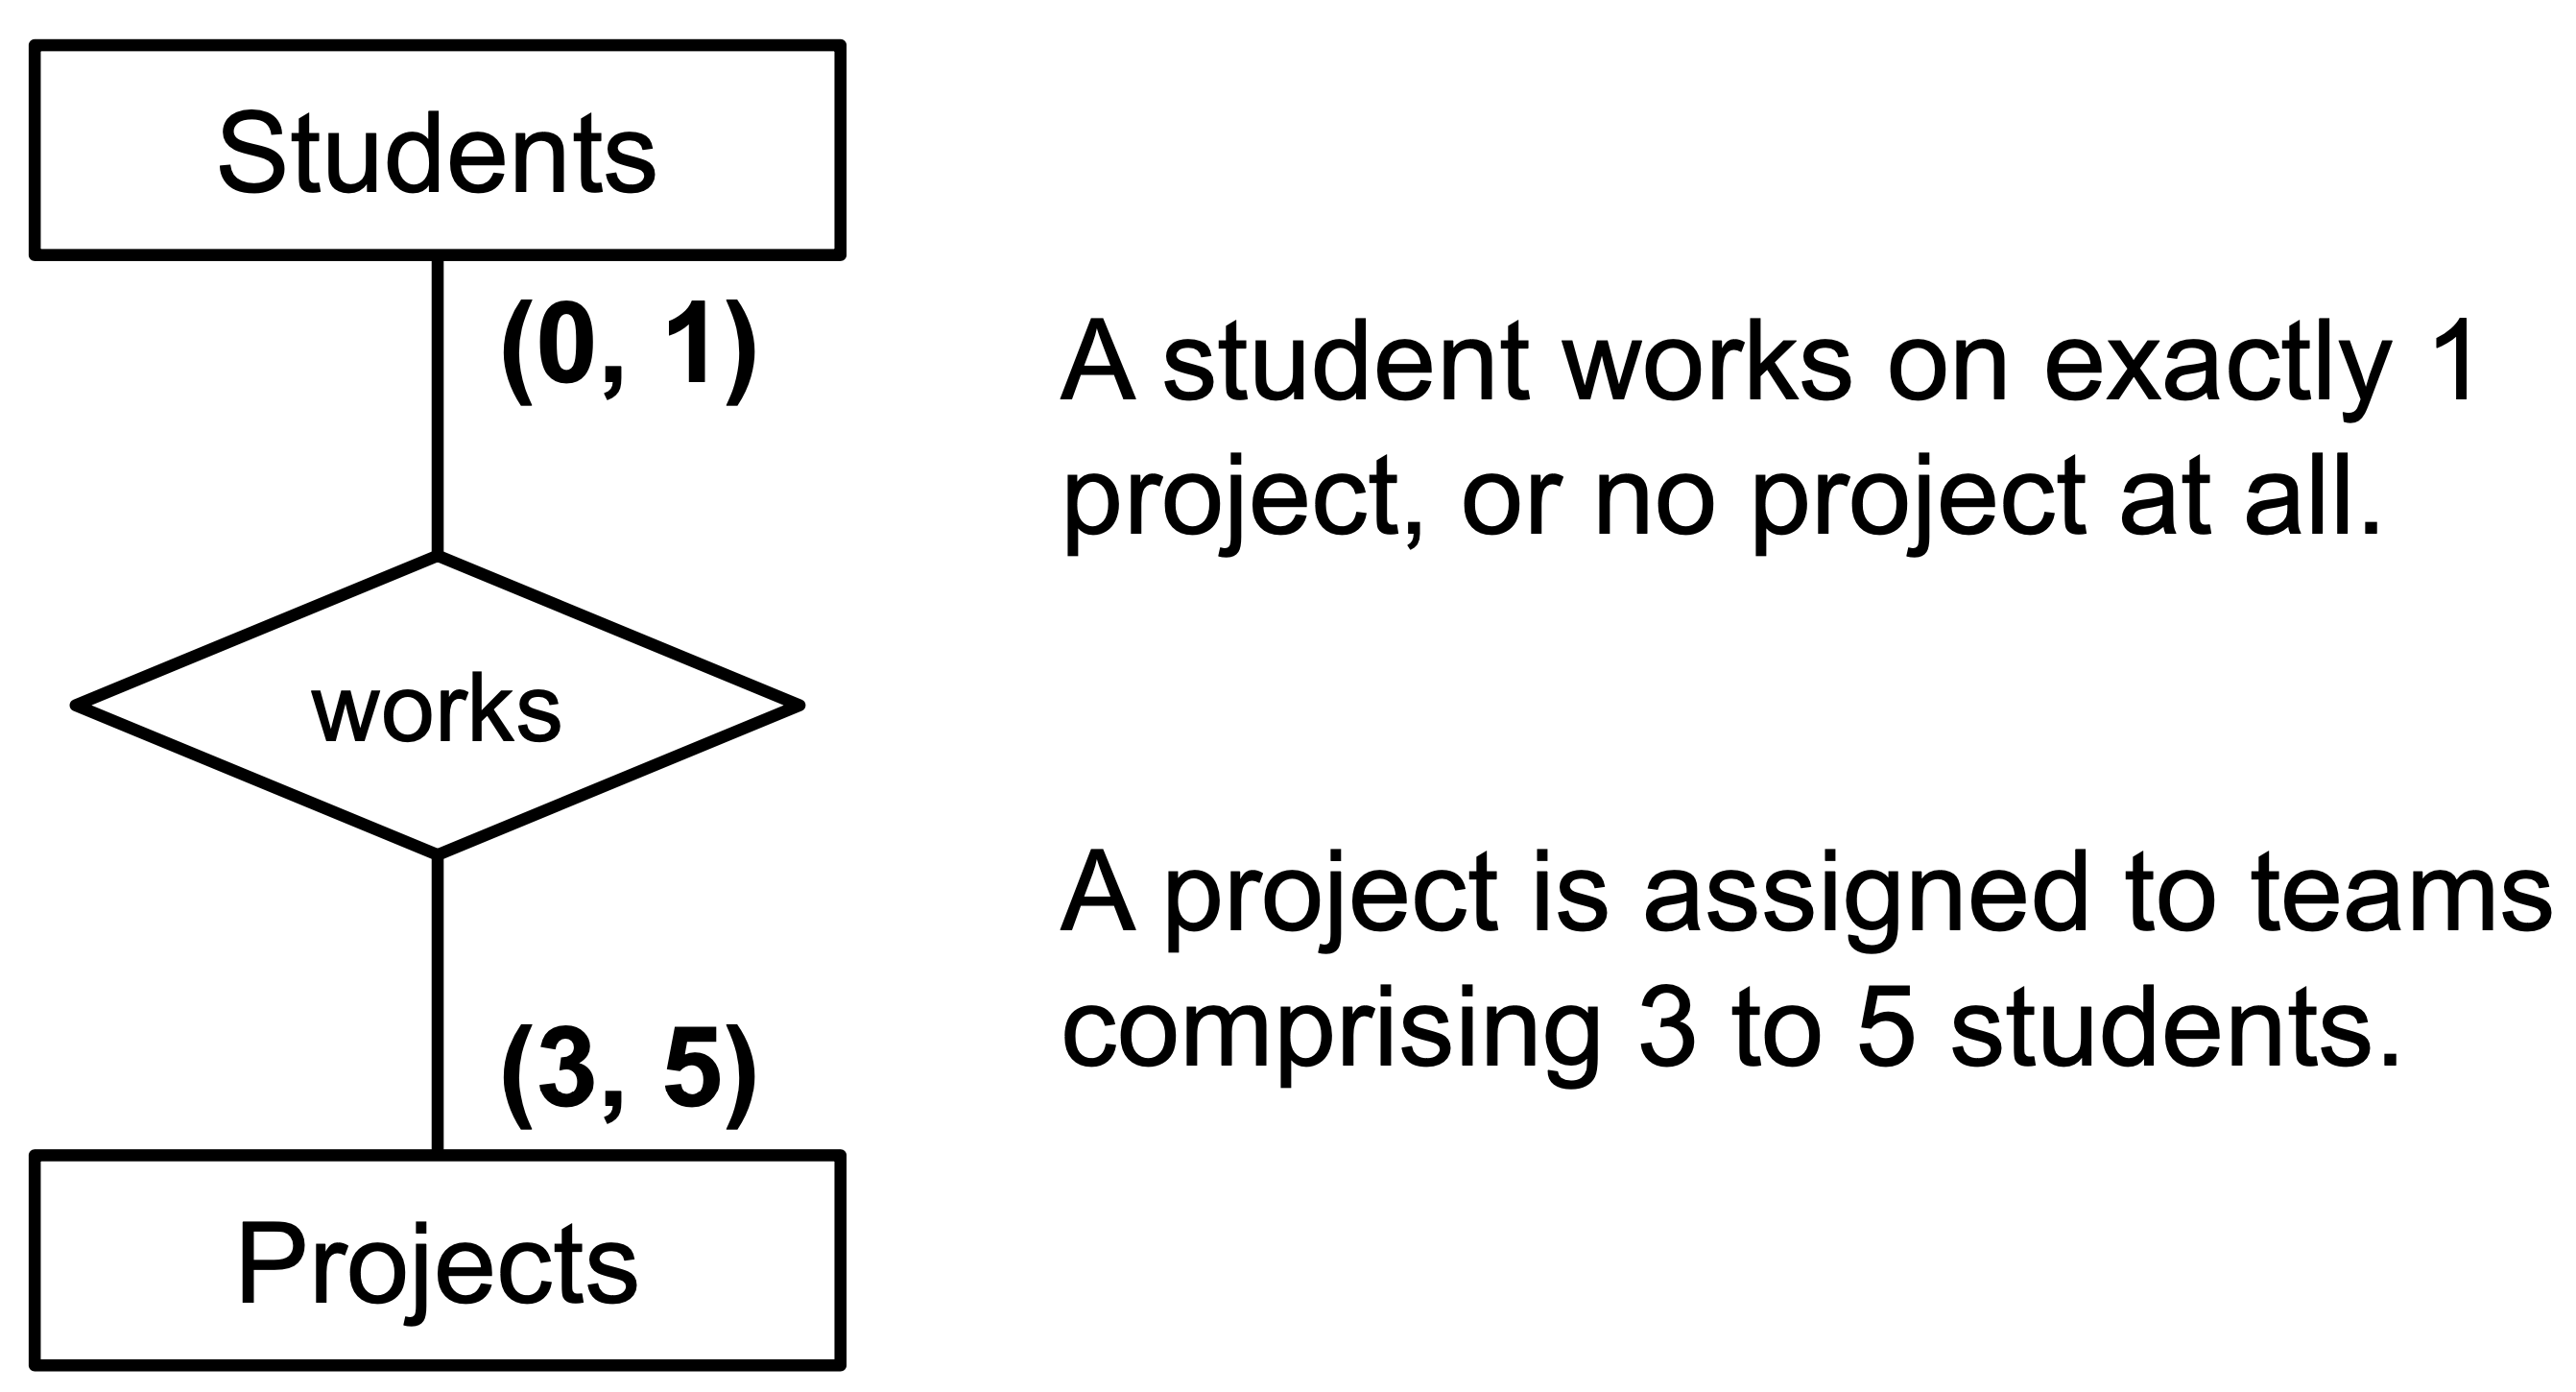
\includegraphics[width=0.4\linewidth]{cs2102-alternative-representation-minmax.png} 
  \end{tightcenter}

  \section{04-1. RELATIONAL MAPPING} 
  \begin{itemize}
    \item entity set $\rightarrow$ table
    \item handling composite/multivalued attributes
      \begin{enumerate}
        \item convert to a set of single-valued attributes (e.g. phone $\rightarrow$ phone1, phone2)
        \item additional table with FK constraint (e.g. PhoneNumbers with user\_id, phone)
        \item convert to one single-valued attribute (e.g. string containing everything)
      \end{enumerate}
  \end{itemize}

  \section{04-2. EXTENDED CONCEPTS}
  \subsection{ISA Hierarchy}
  \begin{itemize}
    \item "is a" relationship used to model generalisation/specialisation of entity sets
    \item every entity in a subclass is an entity in its superclass
      \begin{itemize}
        \item each subclass has specific attributes and/or relationships
      \end{itemize}
  \end{itemize}
  \subsubsection{constraints}
  \begin{itemize}
    \item \definition{overlap contraint} a superclass entity can belong to \textbf{multiple} subclasses
    \item \definition{covering constraint} a superclass entity \textbf{has to} belong to a subclass
  \end{itemize}
  \begin{tightcenter}
    \begin{minipage}[c]{0.45\linewidth}
      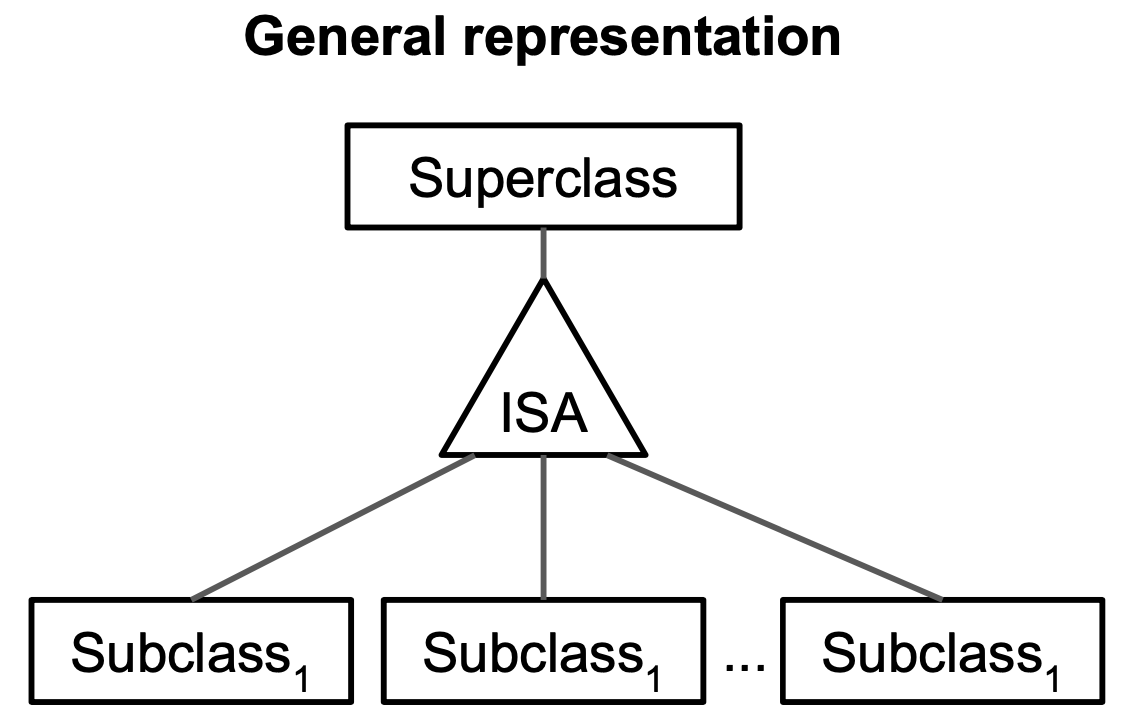
\includegraphics[width=0.95\linewidth]{cs2102-isa-hierarchy-general.png} 
    \end{minipage}
    \begin{minipage}[c]{0.45\linewidth}
      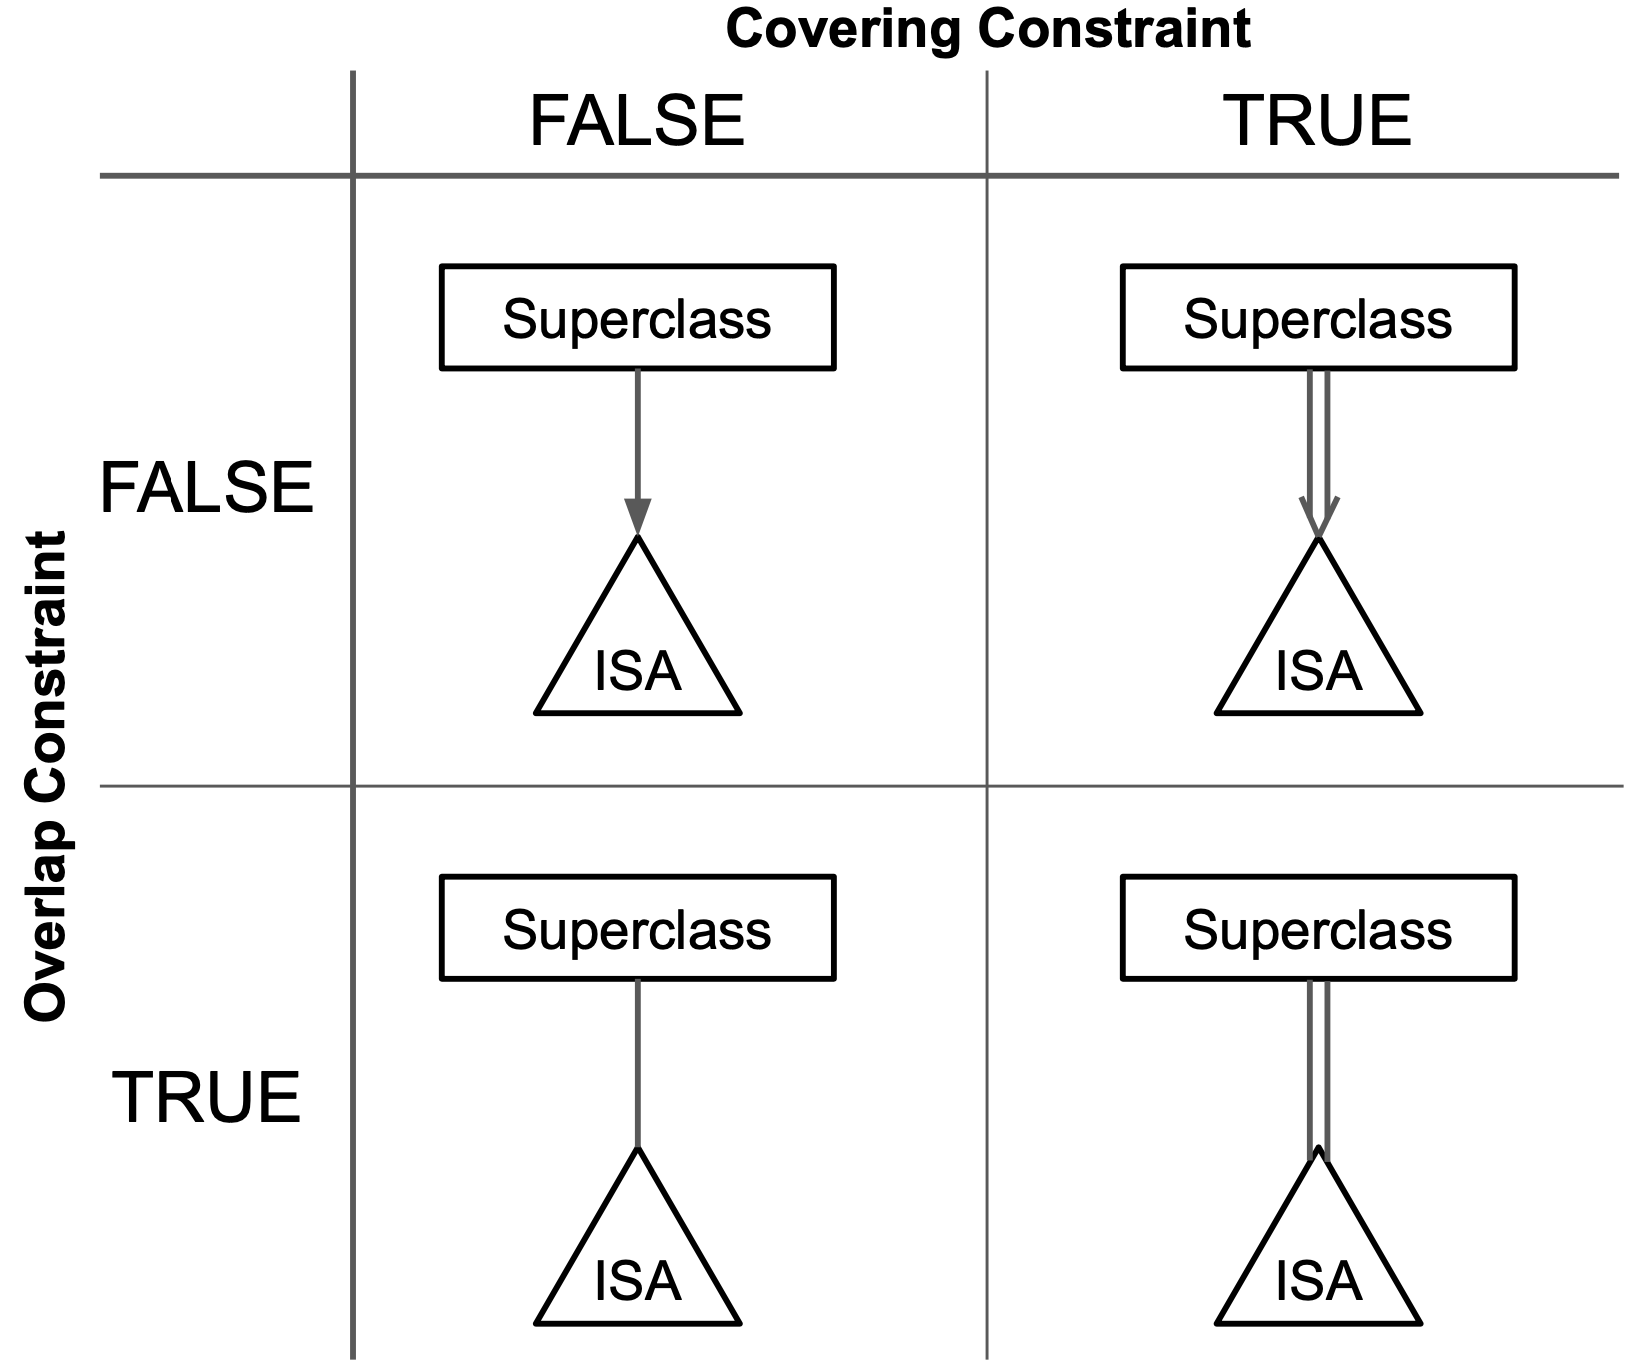
\includegraphics[width=0.95\linewidth]{cs2102-isa-hierarchy-notations.png} 
    \end{minipage}
  \end{tightcenter}

  \subsection{Aggregation}
  \begin{itemize}
    \item abstraction that treats relationships as higher-level entities
      \begin{itemize}
        \item e.g. treating 2 entities + 1 relationship as an entity set
      \end{itemize}
  \end{itemize}
  \begin{minipage}[c]{0.68\linewidth}
    \begin{lstlisting}[style=mySQL]
CREATE TABLE Uses (
  gid INTEGER,
  sid CHAR(20),
  pname VARCHAR(50),
  hours NUMERIC,
  PRIMARY KEY (gid, sid, pname),
  FOREIGN KEY (gid) REFERENCES GPUs (gid),
  FOREIGN KEY (sid, pname) REFERENCES works (sid, pname)
);
    \end{lstlisting}
  \end{minipage}
  \begin{minipage}[c]{0.3\linewidth}
    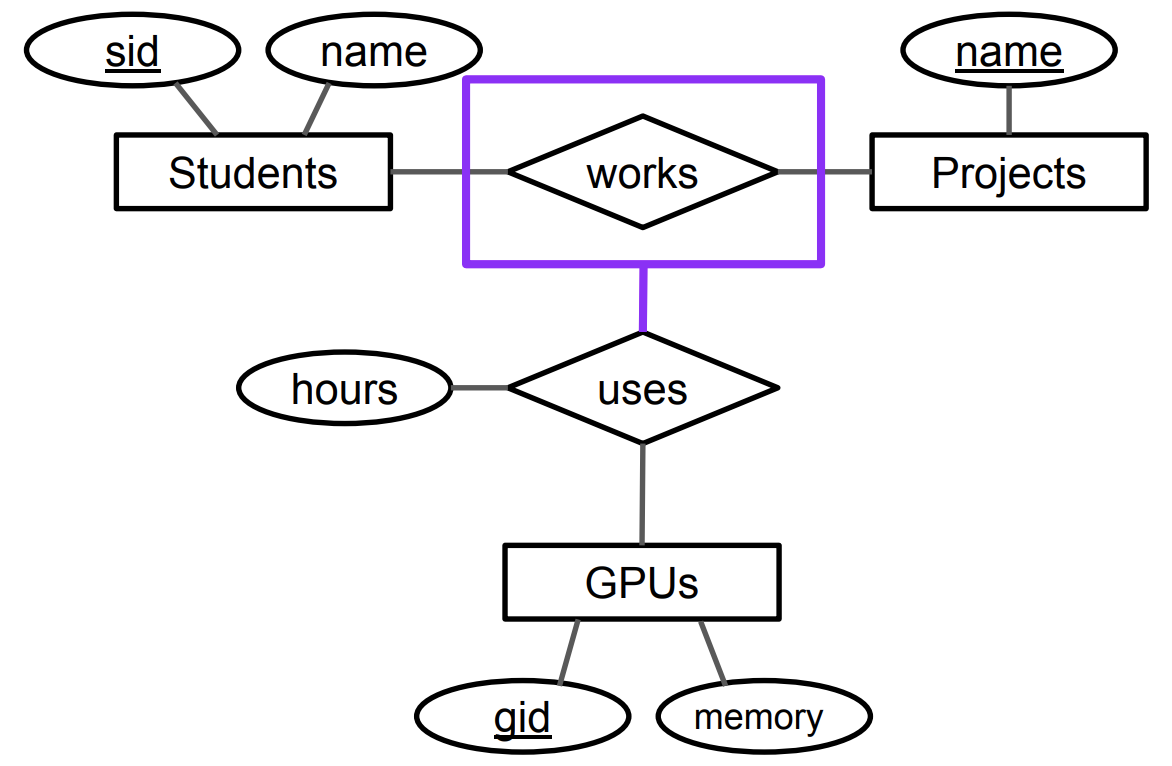
\includegraphics[width=0.98\linewidth]{cs2102-aggregation-example.png} 
  \end{minipage}

  \section{05. SQL (QUERYING A DATABASE)}
  \begin{itemize}
    \item \definition{DQL} data query language
    \item duplicate tuples are allowed!
      \begin{itemize}
        \item use \code{DISTINCT} to eliminate duplicates
      \end{itemize}
  \end{itemize}
  \begin{minipage}[c]{0.3\linewidth}
    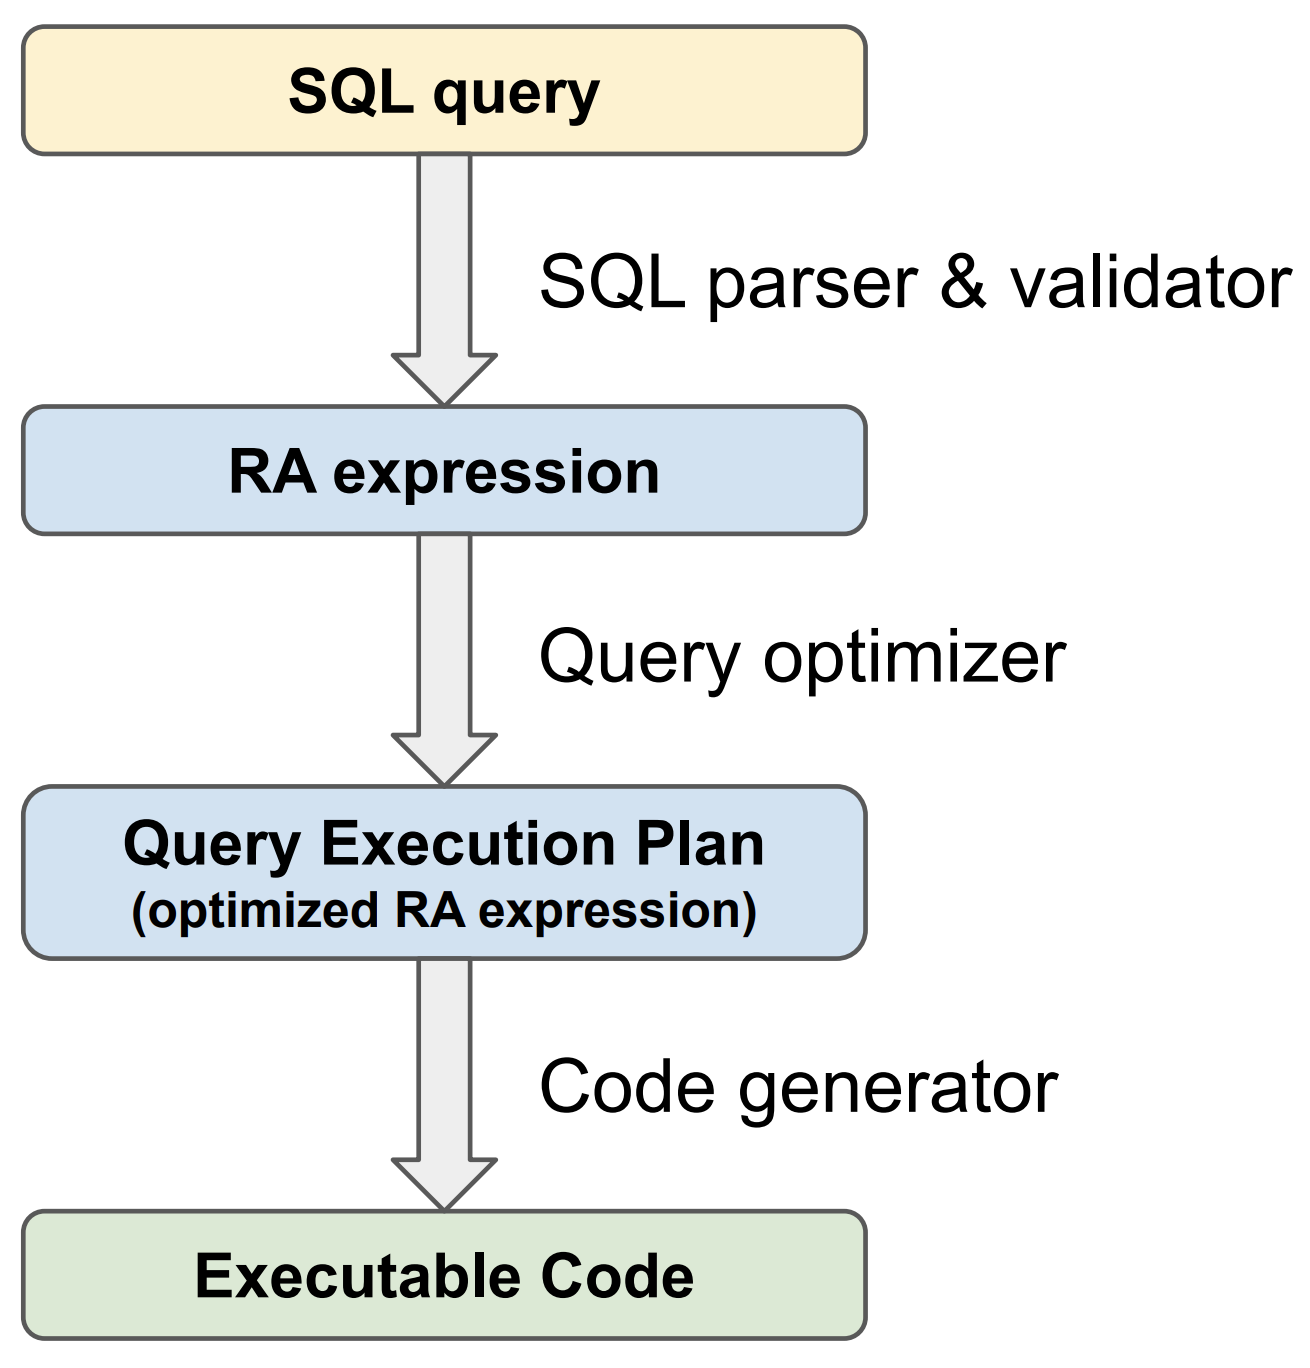
\includegraphics[width=0.9\linewidth]{cs2102-sql-execution-diagram.png} 
  \end{minipage}
  \begin{minipage}[c]{0.5\linewidth}
    \textbf{SELECT DISTINCT} $a_1, a_2, \dots, a_m$ \\* 
    \textbf{FROM} $r_1, r_2, \dots, r_n$ \\* 
    \textbf{WHERE} $c$

    \begin{tightcenter}
      $\Rightarrow$ corresponds to:
      \( {\displaystyle{\pi_{a_1, a_2, \dots, a_m} (\sigma_c(r_1 \times r_2 \times \dots \times r_n)) }} \) 
    \end{tightcenter}
  \end{minipage}

  \subsection{SELECT clause}
  \begin{itemize}
    \item wildcard \code{*} - include all attributes
    \item \code{expr \textbf{BETWEEN} <lower> \textbf{AND} <upper>} - basic value range conditions
      \begin{lstlisting}[style=mySQL]
SELECT * FROM countries 
WHERE (continent = 'Asia' OR continent = 'Europe')
  AND (population BETWEEN 500 AND 600);
      \end{lstlisting}
    \item \code{\textbf{||}} - concatenate strings
      \begin{lstlisting}[style=mySQL]
SELECT name, '$S' || ROUND((gdp/population) * 1.35) AS gdp_per_capita
FROM countries;
      \end{lstlisting}
    \item \code{\textbf{SELECT DISTINCT}} - remove duplicates
      \begin{itemize}
        \item tuples $(n_1, c_1)$ and $(n_2, c_2)$ are considered distinct 
          \\* $\iff$ \code{\textbf{$n_1$ IS DISTINCT FROM $n_2$}} $\lor$ \code{\textbf{$c_1$ IS DISTINCT FROM $c_2$}}
      \end{itemize}
  \end{itemize}

  \subsection{WHERE clause}
  \begin{itemize}
    \item \code{IS (NOT) NULL} 
      \begin{itemize}
        \item evaluates to true: \code{$null$ IS NULL}
        \item evaluates false: \code{$null$ = NULL} (unknown), \code{$null$ <> NULL}
      \end{itemize}
    \item \code{(NOT) LIKE} - pattern matching
      \begin{itemize}
        \item \code{\_} - match any single character
        \item \code{\%} - match any sequence of zero or more characters
      \end{itemize}
  \end{itemize}

  \subsection{SET Operations} 
  \begin{minipage}[c]{0.63\linewidth}
  \begin{itemize}
    \item \code{UNION}, \code{INTERSECT}, \code{EXCEPT}
      \begin{itemize}
        \item \textcolor{black}{will eliminate duplicate tuples from result}
      \end{itemize}
    \item \code{UNION ALL}, \code{INTERSECT ALL}, \code{EXCEPT ALL}
      \begin{itemize}
        \item \textcolor{black}{will NOT eliminate duplicate tuples from result}
      \end{itemize}
    \item \textcolor{black}{no ordering of tuples}
  \end{itemize}
  \end{minipage}
  \begin{minipage}[c]{0.35\linewidth}
    \begin{lstlisting}[style=mySQL]
(SELECT value FROM R)
UNION
(SELECT value FROM S);
    \end{lstlisting}
  \end{minipage}

  \subsection{JOIN Queries}
  \begin{itemize}
    \item \code{JOIN} - interpreted as \code{INNER JOIN} by default
    \item \code{NATURAL JOIN} - joins based on attribute names
      \begin{itemize}
        \item identical attribute names can be reinforced with renaming
      \end{itemize}
    \item \code{LEFT OUTER JOIN} - same as \code{LEFT JOIN}
      \begin{itemize}
        \item keep only dangling tuples: \code{... WHERE c.country\_iso2 IS NULL;}
      \end{itemize}
    \item complex join queries
    \item equivalent queries:
      \begin{lstlisting}[style=mySQL]
SELECT c.name, n.name 
FROM cities AS c, countries AS n
WHERE c.country_iso2 = n.iso2;

SELECT c.name, n.name
FROM cities c INNER JOIN countries n
  ON c.country_iso2 = n.iso2;

SELECT c.name, n.name
FROM cities c JOIN countries n
  ON c.country_iso2 = n.iso2;
      \end{lstlisting}
  \end{itemize}

  \subsection{Subqueries}
  \begin{itemize}
    \item \definition{table alias} every subquery has to have a name (mandatory \textbf{table alias}) to uniquely identify its attributes
      \begin{itemize}
        \item \textbf{column alias} is optional - \code{AS optional}
        \item must be enclosed in parentheses
      \end{itemize}

    \item \code{\textbf{(NOT) IN}} - returns true if \textit{expr} matches \textbf{any} subquery row
      \begin{itemize}
        \item syntax: \code{expr \textbf{IN} (subquery)}, \code{expr \textbf{NOT IN} (subquery)}
        \item subquery must return \textit{exactly one} column
        \item \code{IN} can typically be replaced with (inner) joins
        \item \code{NOT IN} can typically be replaced with (outer) joins
          \begin{lstlisting}[style=mySQL]
SELECT name FROM COUNTRIES
WHERE name IN (SELECT name FROM cities)
   OR name IN ('Singapore', 'Hong Kong');
          \end{lstlisting}
      \end{itemize}

    \item \code{\textbf{ANY}} - returns true if comparison evaluates to true for \textit{at least one} subquery row
      \begin{itemize}
        \item syntax: \code{expr op \textbf{ANY} (subquery)}
        \item subquery must return \textit{exactly one} column
        \item expression is compared to each subquery row using \code{op} 
          \begin{lstlisting}[style=mySQL]
SELECT name, population FROM countries 
WHERE population < ANY (SELECT population FROM cities
                        WHERE country = 'GB');
          \end{lstlisting}
      \end{itemize}

    \item \code{\textbf{ALL}} - returns true if comparison evaluates to true for \textit{all} subquery rows
      \begin{itemize}
        \item syntax: \code{expr op \textbf{ALL} (subquery)}
          \begin{lstlisting}[style=mySQL]
SELECT name, continent, gdp FROM countries c1
WHERE gdp >= ALL(SELECT gdp FROM countries c2
                 WHERE c2.continent = c1.continent); 
                 -- c1 from outer query
          \end{lstlisting}
      \end{itemize}

    \item \code{\textbf{EXISTS}} - returns true if the subquery returns \textit{at least one} tuple
      \begin{itemize}
        \item syntax: \code{\textbf{EXISTS} (subquery)}, \code{\textbf{NOT EXISTS} (subquery)}
        \item \code{(NOT) EXISTS} subqueries are generally \textbf{correlated}
          \begin{itemize}
            \item uncorrelated $\Rightarrow$ will always give the same result $\Rightarrow$ redundant
          \end{itemize}
          \begin{lstlisting}[style=mySQL]
SELECT n.name FROM countries n
WHERE NOT EXISTS (SELECT * FROM cities c
                  where c.country_iso2 = n.iso2);
                  -- n from outer query
          \end{lstlisting}
      \end{itemize}
  \end{itemize}

  \subsubsection{correlated subquery}
  \begin{itemize}
    \item \definition{correlated subquery} relies on value(s) from outer query
    \item result of subquery depends on value of outer query
      \begin{itemize}
        \item potential performance issues (slow)
        \item potential naming ambiguity - use table aliases
      \end{itemize}
    \item \textbf{scoping rules}
      \begin{itemize}
        \item a table alias declared in subquery $Q$ can only be used in $Q$ or subqueries nested within $Q$
        \item if the same table alias is declared both in $Q$ and in an outer query (or undeclared), the declaration in Q is applied.
          \begin{itemize}
            \item aka when unsure, apply the smallest scope ("inner to outer")
          \end{itemize}
      \end{itemize}
  \end{itemize}

  \subsubsection{scalar subqueries}
  \begin{itemize}
    \item \definition{scalar subquery} returns a \textbf{single} value (1 row 1 column)
    \item can be used as an expression in queries
  \end{itemize}

  \subsubsection{row constructors}
  \begin{itemize}
    \item allow subqueries to return more than one attribute/column
      \begin{itemize}
        \item number of attributes/columns in the row constructor must match that of the subquery
      \end{itemize}
    \item e.g. find all countries with higher population \textit{or} gdp than France \textit{or} Germany
  \end{itemize}
  \begin{lstlisting}[style=mySQL]
SELECT name, population AS pop, gdp FROM countries
WHERE ROW(pop, gdp) > ANY(SELECT population, gdp 
                          FROM countries
                          WHERE name IN ('Germany', 'France'));
  \end{lstlisting}

  \subsubsection{equivalent subqueries}
  \begin{itemize}
    \item \code{expr \textbf{IN} (subquery)} $\, \equiv \,$ \code{expr = \textbf{ANY} (subquery)}
    \item \code{expr1 op \textbf{ANY} (\textbf{SELECT} expr2 \textbf{FROM} ... \textbf{WHERE} ...)} 
      \\* $\, \equiv \,$ \code{\textbf{EXISTS} (\textbf{SELECT} * \textbf{FROM} ... \textbf{WHERE} ... \textbf{AND} expr1 op expr2)}
  \end{itemize}

  \subsection{Sorting}
  \begin{itemize}
    \item \code{ORDER BY} - sort by attribute(s), \code{ASC}/\code{DESC} 
    \item e.g. \code{ORDER BY n.name ASC, c.population DESC}
      \begin{itemize}
        \item second criteria only affects result if first criteria has ambiguity
      \end{itemize}
  \end{itemize}

  \subsection{Rank-based Selection}
  \begin{itemize}
    \item \code{LIMIT k} - return the first $k$ tuples of the result table
    \item \code{OFFSET i} - specify the position of the "first" tuple to be considered
      \begin{lstlisting}[style=mySQL]
-- e.g. find the "second" top 5 countries by GDP per capita
SELECT name, (gdp/population) AS gdp_per_capita FROM countries
ORDER BY gdp_per_capita DESC 
OFFSET 5 LIMIT 5;
      \end{lstlisting}
  \end{itemize}

  \section{06-1. SQL (AGGREGATION)}

  \begin{itemize}
    \item compute a single value from a set of tuples
    \item NOT allowed in WHERE
    \item e.g. \code{MIN()}, \code{MAX()}, \code{AVG()}, \code{COUNT()}, \code{SUM()} 
      \begin{lstlisting}[style=mySQL]
SELECT MIN(population) as lowest,
       MAX(population) as highest,
       SUM(population) as world
FROM countries;
      \end{lstlisting}
  \end{itemize}

  \subsection{handling null values}
  \begin{tightcenter}
    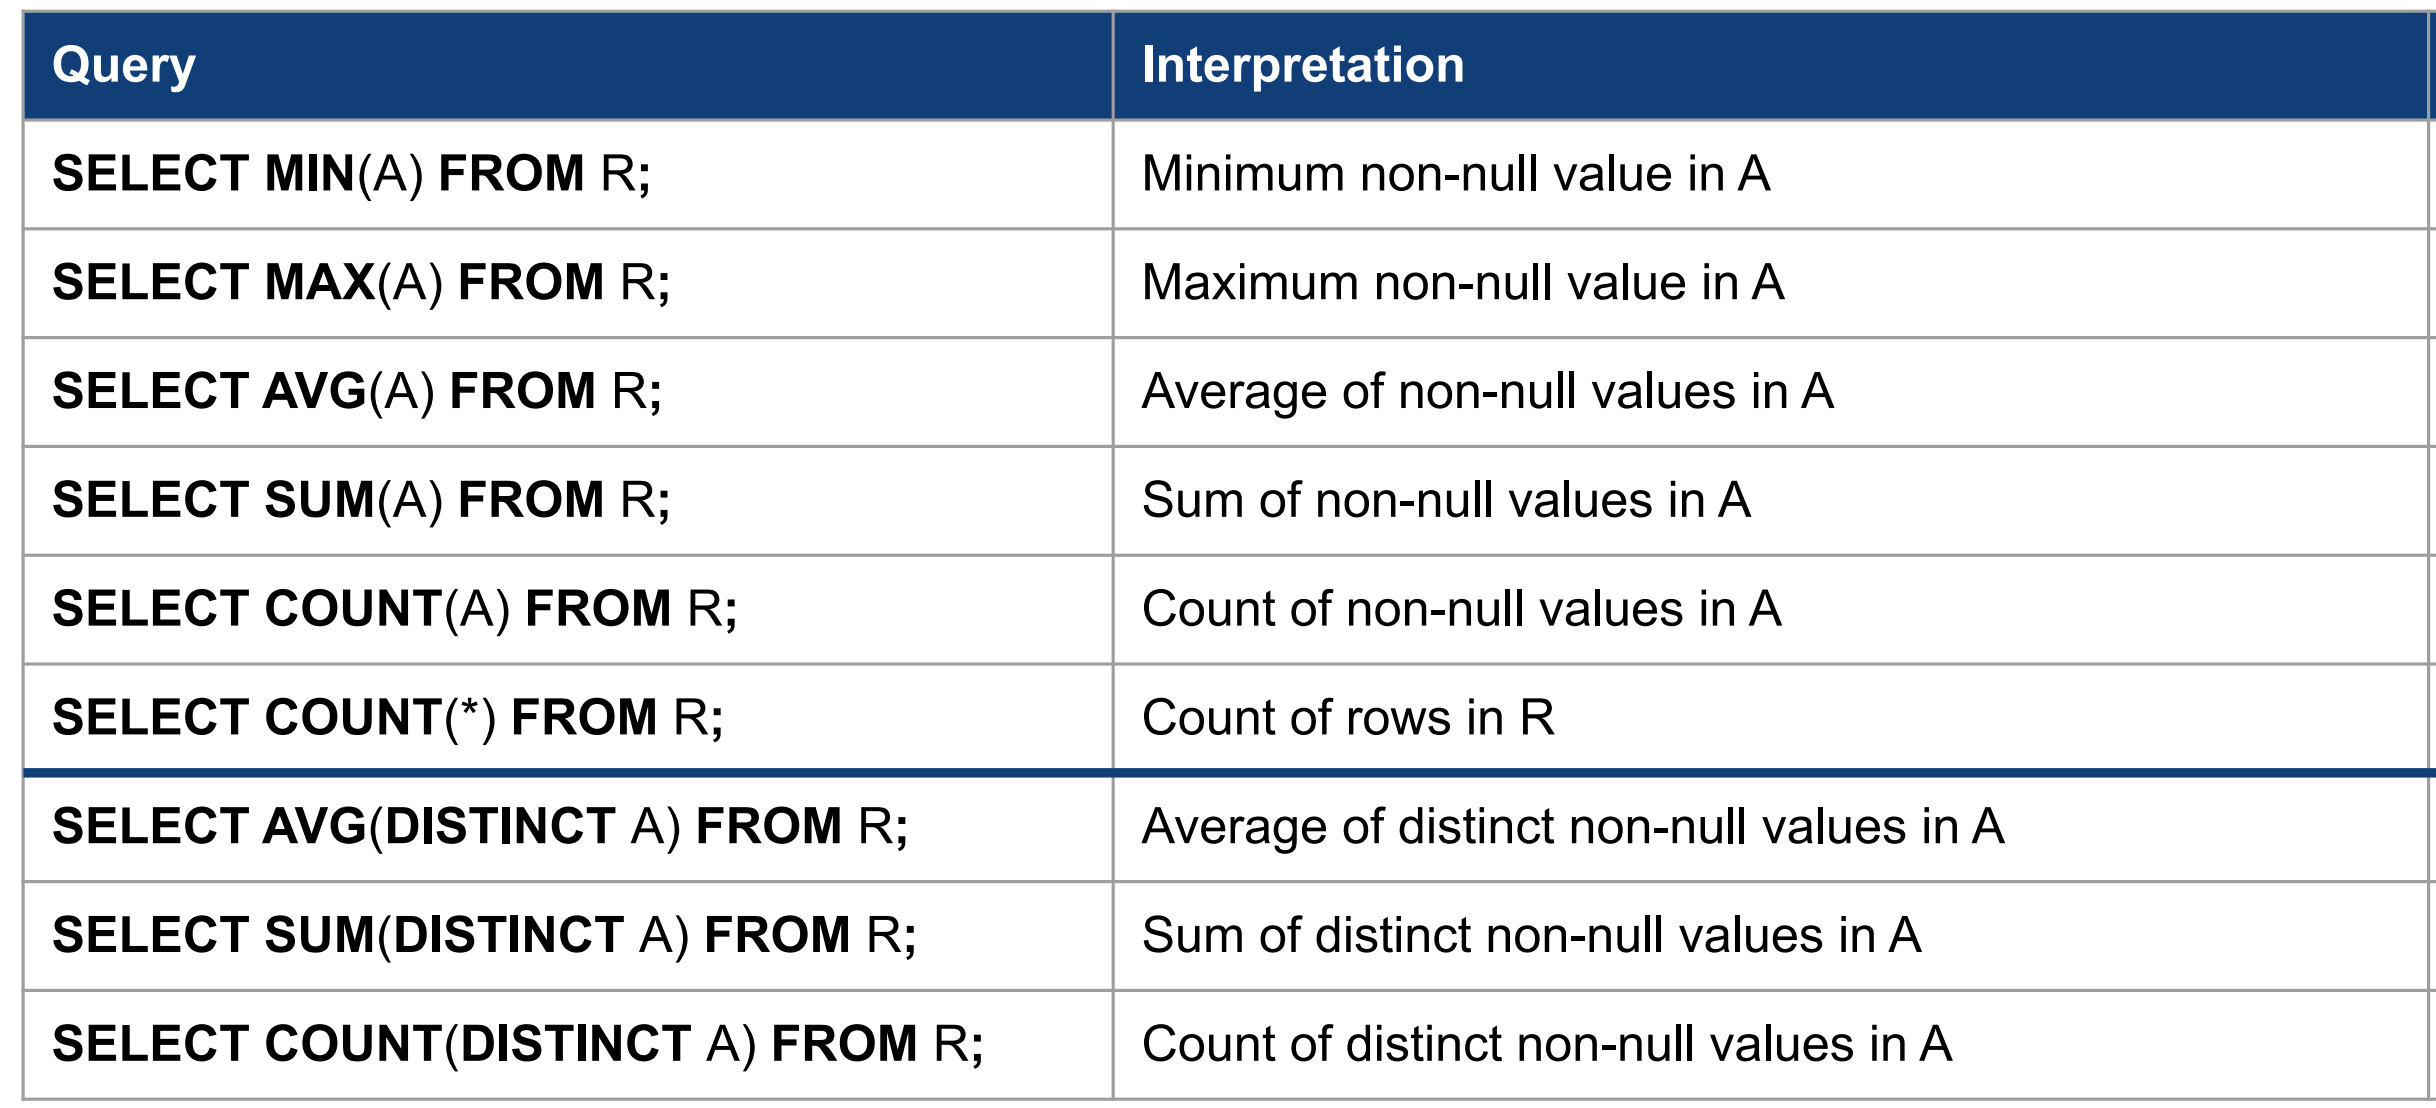
\includegraphics[width=0.9\linewidth]{cs2102-aggregation-functions-summary.png} 
  \end{tightcenter}
  Let $R$ be an empty relation; let $S$ be a non-empty relation with $n$ tuples but ONLY null values for $A$.
  \begin{tightcenter}
    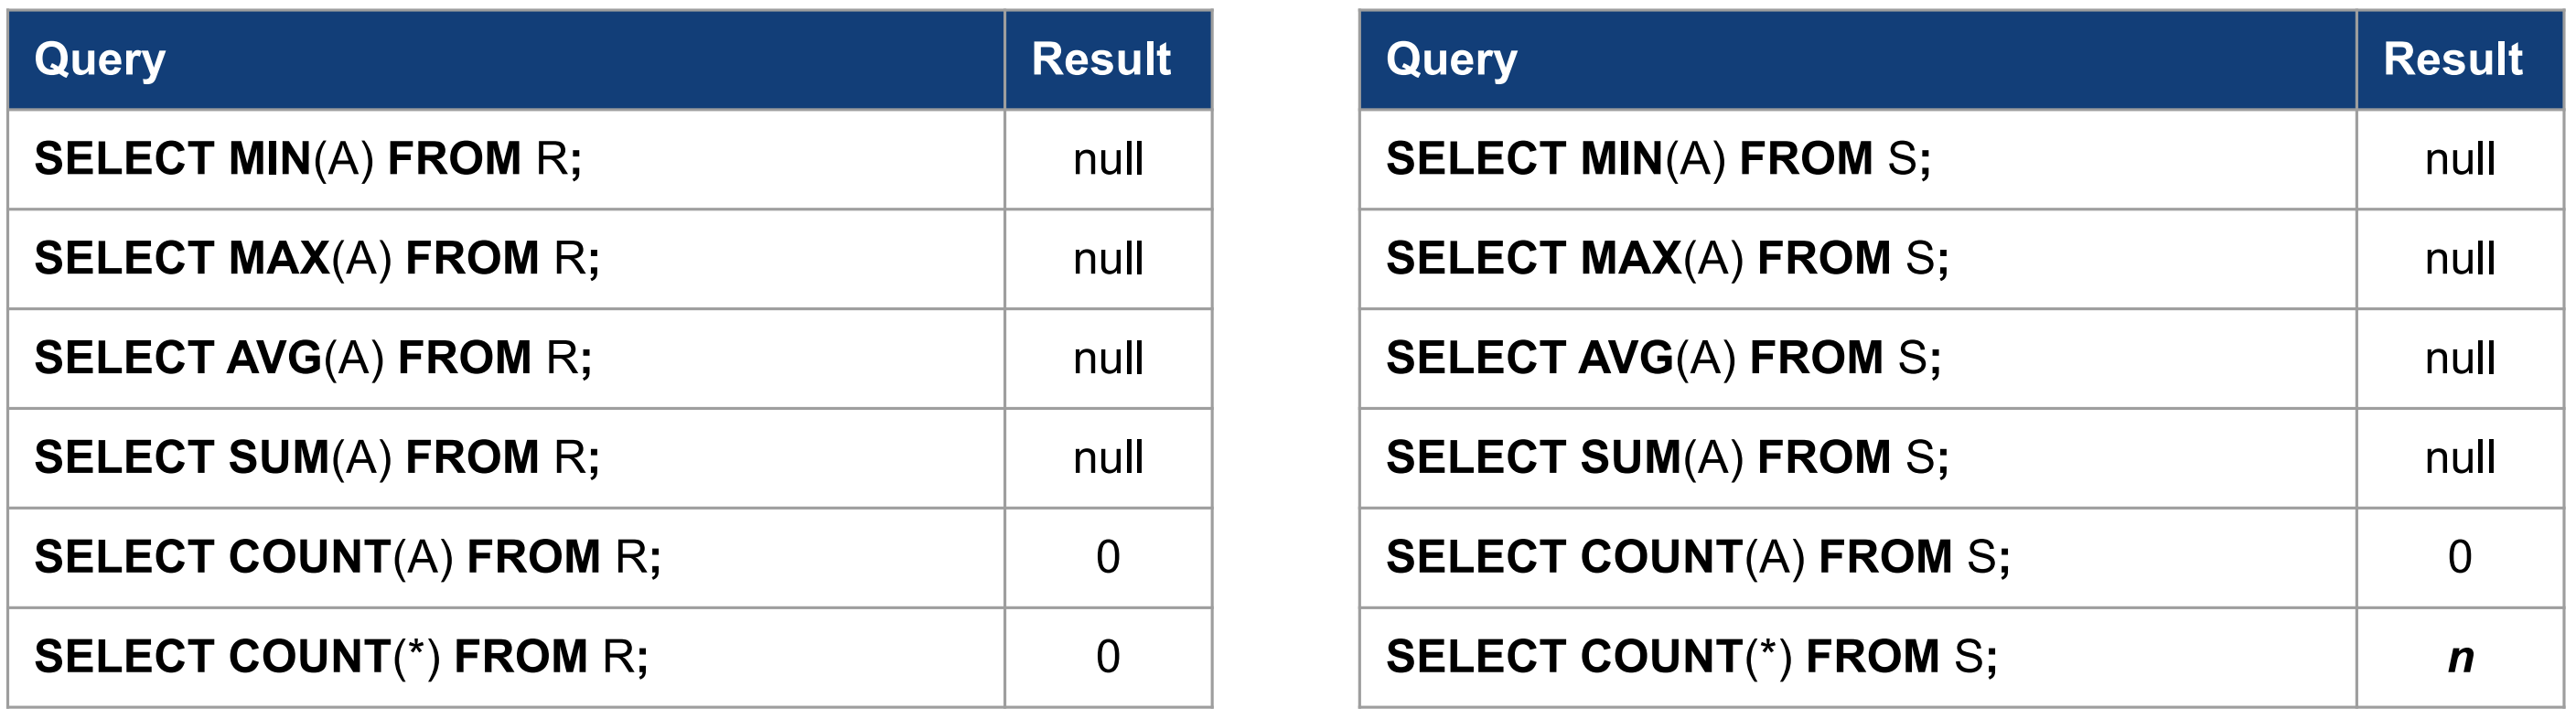
\includegraphics[width=0.9\linewidth]{cs2102-aggregation-function-null.png} 
  \end{tightcenter}

  \subsection{signatures}
  \begin{itemize}
    \item \code{\textbf{MIN}}, \code{\textbf{MAX}} : defined for all data types, returns same data type as input
    \item \code{\textbf{SUM}} : defined for all \textbf{numeric} data types
      \begin{itemize}
        \item \code{\textbf{SUM}(INTEGER) -> BIGINT}, \code{\textbf{SUM}(REAL) -> REAL}
      \end{itemize}
    \item \code{\textbf{COUNT}} : defined for all datatypes; \code{\textbf{COUNT}(...) -> BIGINT}
  \end{itemize}

  \subsection{GROUP BY}
  \begin{itemize}
    \item given \code{GROUP BY $a_1, a_2, \dots, a_n$}, 2 tuples $t$ and $t'$ belong to the same group if 
      \\* $\forall k \in (1, n)$,  \code{(t.a$_k$ \textbf{IS NOT DISTINCT FROM} t'.a$_k$)} evaluates to \code{TRUE}.
    \item logical partition of relation into groups based on values for specified attributes
    \item one result tuple for each group
    \item if column $A_i$ or table $R$ appears in the SELECT clause, one of the following conditions must hold:
      \begin{enumerate}
        \item $A_i$ appears in the GROUP BY clause
        \item $A_i$ appears as input of an aggregation function in the SELECT clause
        \item the primary key of $R$ appears in the GROUP BY clause
      \end{enumerate}
  \end{itemize}
  \begin{lstlisting}[style=mySQL]
-- for each continent, find the lowest, highest and total country population and number of countries
SELECT continent,
  MIN(population) AS lowest,
  MAX(population) AS highest,
  SUM(population) AS overall,
  COUNT(*)        AS number_of_countries,
FROM countries
GROUP BY continent;
  \end{lstlisting}

  \subsubsection{HAVING}
  \begin{itemize}
    \item conditions check for each group defined by \code{GROUP BY} clause
      \begin{itemize}
        \item cannot be used without a \code{GROUP BY} clause
      \end{itemize}
    \item if column $A_i$ of table $R$ apears in the \code{HAVING} clause, one of the following conditions must hold:
      \begin{enumerate}
        \item $A_i$ appears in the GROUP BY clause
        \item $A_i$ appears as input of an aggregation function in the HAVING clause
        \item the primary key of $R$ appears in the GROUP BY clause
      \end{enumerate}
      \begin{lstlisting}[style=mySQL]
-- find all routes served by >12 airlines
SELECT from_code, to_code, COUNT(*) AS num_airlines
FROM routes 
GROUP BY from_code, to_code
HAVING COUNT(*) > 12;
      \end{lstlisting}
  \end{itemize}

  \section{06-2. SQL (CONDITIONAL EXPRESSION)}
  \subsection{CASE}
  \begin{itemize}
    \item generic conditional expression, similar to if/else
    \item two basic ways of formulating CASE expressions:
  \end{itemize}
  \begin{minipage}[c]{0.48\linewidth}
    \begin{lstlisting}[style=mySQL]
CASE
  WHEN condition1 THEN result1
  WHEN condition2 THEN result2
  ...
  WHEN condition_n THEN result_n
  ELSE result0
END
    \end{lstlisting}
  \end{minipage}
  \,
  \begin{minipage}[c]{0.48\linewidth}
    \begin{lstlisting}[style=mySQL]
CASE expression
  WHEN value1 THEN result1
  WHEN value2 THEN result2
  ...
  WHEN condition_n THEN result_n
  ELSE result0
END
    \end{lstlisting}
  \end{minipage}

  \subsection{COALESCE}
  \begin{itemize}
    \item \code{COALESCE(val1, val2, ...)} returns the first NON-NULL value in the list of input arguments
    \item returns NULL if all values in the list of input arguments are NULL
    \item e.g. \code{SELECT COALESCE(null, null, 1, null, 2) -> 1}
  \end{itemize}
  \begin{lstlisting}[style=mySQL]
-- find the number of cities for each city type;
-- consider cities with NULL for capital as 'other'
SELECT capital, COUNT(*) AS city_count FROM
  (SELECT COALESCE(capital, 'other') AS capital FROM cities) t
GROUP BY capital;
  \end{lstlisting}

  \subsection{NULLIF}
  \begin{itemize}
    \item \code{NULLIF(val1, val2)} returns NULL if \code{val1 = val2}; otherwise return \code{val1}
    \item common use case: convert special values to NULL
  \end{itemize}
  \begin{lstlisting}[style=mySQL]
-- select min and average GDP 
-- from a table where unknown GDP is represented as 0
SELECT MIN(NULLIF(gdp, 0)) AS min_gdp, 
       ROUND(AVG(NULLIF(gdp, 0))) AS avg_gdp
FROM countries;
  \end{lstlisting}

  \section{06-3. SQL (STRUCTURING QUERIES)}
  \subsection{Common Table Expressions (CTEs)}
  \begin{itemize}
    \item \textit{temporarily} named query
  \end{itemize}

  \begin{minipage}[c]{0.2\linewidth}
    general syntax:
    \\ \textbf{WITH}
    \\* $\quad$ C$_1$ \textbf{AS} (Q$_1$)
    \\* $\quad$ C$_2$ \textbf{AS} (Q$_2$)
    \\* $\quad \cdots,$ ...,
    \\* $\quad$ C$_n$ \textbf{AS} (Q$_n$)
  \end{minipage}
  \begin{minipage}[c]{0.75\linewidth}
    \begin{lstlisting}[style=mySQL]
WITH CTE_name AS 
  -- <CTE BODY>
  (SELECT n.name AS country, ...
   FROM ...
   WHERE ...)
  -- </CTE BODY>
SELECT i.country, ...
FROM CTE_name i   /* CTE usage */ 
  LEFT OUTER JOIN routes r N i.code = r.to_code
...
    \end{lstlisting}
  \end{minipage}

  \begin{itemize}
    \item general syntax
      \begin{itemize}
        \item each $C_i$ is the name of a temporary table defined by query $Q_i$ 
        \item each $C_i$ can reference any other $C_j$ that has been declared \textit{before} $C_i$ 
        \item SQL statement $S$ can reference any possible subset of all $C_i$
      \end{itemize}
  \end{itemize}

  \subsection{Views}
  \begin{itemize}
    \item \textit{permanently} named \textbf{query} (virtual relation)
      \begin{itemize}
        \item query is stored (not the query result) $\Rightarrow$ re-executed whenever it is used
      \end{itemize}
    \item can be used like normal tables
      \begin{itemize}
        \item no restriction when used in SELECT statements
        \item restrictions when using INSERT/UPDATE/DELETE
      \end{itemize}
  \end{itemize}
  \begin{lstlisting}[style=mySQL]
CREATE VIEW ViewName AS
  SELECT ...
  FROM ...
  WHERE ... ;
  \end{lstlisting}

  \subsection{RECURSIVE QUERIES}
  \begin{itemize}
    \item using CTEs and \code{RECURSIVE}
  \end{itemize}
  \begin{lstlisting}[style=mySQL]
WITH RECURSIVE CTE_name (col_a, col_b, col_c) AS (
  SELECT ... , 0 as counter
  FROM ...  WHERE ...
  UNION ALL
  SELECT ..., cte.counter + 1
  FROM CTE_name cte, ... WHERE ...
  AND cte.counter < 3  /* base case */
)
SELECT DISTINCT counter, ... 
FROM CTE_name
ORDER BY counter ASC;
  \end{lstlisting}

  \subsection{UNIVERSAL QUANTIFICATION}
  \begin{itemize}
    \item no direct support for universal quantification (e.g. find users who have visited \textit{all} countries)
      \begin{itemize}
        \item SQL only supports \textit{existential} quantification (EXISTS)
      \end{itemize}
    \item possible workarounds:
  \end{itemize}
  \begin{multicols}{2}
    \begin{lstlisting}[style=mySQL]
SELECT n.iso2
FROM countries n
WHERE NOT EXISTS (SELECT 1
 FROM visited v
 WHERE v.iso2 = n.iso2
AND v.user_id = x);
    \end{lstlisting}

    \begin{lstlisting}[style=mySQL]
  SELECT u.user_id, u.name
  FROM users u, visited v
  WHERE u.user_id = v.user_id
  GROUP BY u.user_id
  HAVING COUNT(*) = (SELECT COUNT(*) FROM countries);
    \end{lstlisting}
  \end{multicols}

  \section{07. PL/pgSQL}
  \begin{itemize}
    \item SQL-based Procedural Language implemented by PostgreSQL
  \end{itemize}

  \subsection{Functions}
  \begin{itemize}
    \item \code{CREATE OR REPLACE} - best practice (just \code{CREATE} is possible as well)
    \item \code{<type>}: all data types in SQL, a tuple, a set of tuples, custom tuples, triggers
      \begin{itemize}
        \item to return nothing: \code{RETURNS VOID AS ...}
      \end{itemize}
    \item main body of function is enclosed within \code{\$\$}
    \item functions are compiled $\rightarrow$ validity is not checked whenever you call the function
      \begin{itemize}
        \item vs CTE views - validity is checked by the engine every time it's called
      \end{itemize}
  \end{itemize}
  \begin{lstlisting}[style=mySQL]
-- define function
CREATE OR REPLACE FUNCTION function_name(x INT, y INT)
RETURNS CHAR(1) AS $$
  SELECT CASE 
    WHEN x >= 70 THEN 'A'
    WHEN y >= 60 THEN 'B'
    ELSE 'C'
  END
$$ LANGUAGE sql;

-- call function
SELECT function_name(65, 67);  /* returns a composite type, tuple */
SELECT * FROM function_name(66, 68);  /* returns a table */
SELECT name, function_name(marks1, marks2) AS grade FROM Scores;
  \end{lstlisting}

  \subsubsection{returning a set of tuples}
  \begin{itemize}
    \item by default, a function will only return the first tuple (similar to using \code{LIMIT 1})
    \item to return a set of tuples: \code{SETOF}
      \begin{lstlisting}[style=mySQL]
-- returns a set of tuples
CREATE OR REPLACE FUNCTION GradeStudents 
  (Grade CHAR(1))
RETURNS SETOF Scores AS $$ 
  SELECT *
  FROM Scores
  WHERE convert(Mark) = Grade;
$$ LANGUAGE sql;
      \end{lstlisting}
  \end{itemize}

  \subsubsection{returning a custom tuple}
  \begin{itemize}
    \item specify \code{IN} and \code{OUT} for input and output parameters
      \begin{lstlisting}[style=mySQL]
-- returns a tuple (Mark, Count)
CREATE OR REPLACE FUNCTION CountGradeStudents
  (IN Grade CHAR(1) OUT Mark CHAR(1), OUT Count INT)
RETURNS RECORD AS $$  /* use SETOF to return all tuples */
  SELECT Grade, COUNT(*)
  FROM Scores
  WHERE convert(Mark) = Grade;
$$ LANGUAGE sql;

-- call the function
SELECT CountGradeStudents('C');
      \end{lstlisting}
  \end{itemize}

  \subsection{Procedures}
  \begin{itemize}
    \item no return value
  \end{itemize}
  \begin{lstlisting}[style=mySQL]
-- define a procedure
CREATE OR REPLACE PROCEDURE UpdateMark
  (IN amount INTEGER)
AS $$
  UPDATE Scores SET Mark = Mark + amount;
  ALTER TABLE Scores ADD COLUMN IF NOT EXISTS
    Grade CHAR(1) DEFAULT NULL;
  SELECT * FROM Scores;
$$ LANGUAGE sql;

-- call the procedure
CALL UpdateMark(1);
  \end{lstlisting}

  \subsection{Variables}
  \begin{lstlisting}[style=mySQL]
CREATE OR REPLACE FUNCTION splitMarks  /* same for PROCEDURE */
  (IN name1 VARCHAR(20), IN name2 VARCHAR(20), OUT mark1 INT, OUT mark2 INT)
RETURNS TABLE(mark1 INT, mark2 INT) AS $$  /* return multiple tuples */
DECLARE
  newmark INT := 0;
BEGIN
  SELECT mark INTO mark1 FROM Scores WHERE name = name1;  /* selects into a mark1 variable */
  SELECT mark INTO mark2 FROM Scores WHERE name = name2;  /* selects into a mark2 variable */

  newmark := (mark1 + mark2) / 2;

  UPDATE Scores SER mark = newmark WHERE name = name1 OR name = name2;
  -- does NOT exit the function:
  RETURN QUERY SELECT mark1, mark2;  /* returns values */
  -- does NOT exit the function:
  RETURN NEXT;  /* returns the defined output parameters */
  -- returns output params and EXITS the function:
  RETURN;  /* optional */
END;
$$ LANGUAGE plpgsql;  /* not sql */
  \end{lstlisting}

  \subsubsection{Return statements}
  \begin{itemize}
    \item without \code{RETURN}, function will end naturally and return output params
    \item \code{RETURN;} - returns output params and \textbf{exits} the function
      \item \code{RETURN QUERY <SELECT ...>;} - appends queried tuples to output table; does not exit function
        \item \code{RETURN NEXT;} - appends output params to output table; does not exit function
  \end{itemize}

  \subsection{Control Flow}
  \subsubsection{Conditionals}
  \begin{lstlisting}[style=mySQL]
CREATE OR REPLACE FUNCTION splitMarks  /* same for PROCEDURE */
  (IN name1 VARCHAR(20), IN name2 VARCHAR(20), OUT mark1 INT, OUT mark2 INT)
RETURNS TABLE(mark1 INT, mark2 INT) AS $$  
DECLARE
  newmark INT := 0;
BEGIN
  -- <SELECT statements />
  newmark := (mark1 + mark2) / 2;
  IF x > 60 THEN     x := x / 2;
  ELSIF x > 50 THEN  x := x - 20;
  ELSE               x := x - 10;
  END IF;
  -- <UPDATE statements />
  RETURN QUERY SELECT mark1, mark2;  /* returns values */
END;
  \end{lstlisting}

  \subsubsection{While}
  \begin{lstlisting}[style=mySQL]
BEGIN
  -- <SELECT statements />
  x := (mark1 + mark2) / 2;
  WHILE x > 30 LOOP
    x := x / 2;
  END LOOP;
  -- <UPDATE statements />
  RETURN QUERY SELECT mark1, mark2;  
END;
  \end{lstlisting}

  \subsubsection{Exit When}
  \begin{itemize}
    \item equivalent to \code{while True: if (cond): break;}
  \end{itemize}
  \begin{lstlisting}[style=mySQL]
BEGIN
  -- <SELECT statements />
  LOOP
    EXIT WHEN x < 30;
    x := x / 2;
  END LOOP;
  -- <UPDATE statements />
  RETURN QUERY SELECT mark1, mark2;  
END;
  \end{lstlisting}

  \subsubsection{Foreach}
  \begin{lstlisting}[style=mySQL]
DECLARE
  x INT := 0; d INT; denoms INT[] := ARRAY[1, 2, 3];
BEGIN
  -- <SELECT statements />
  FOREACH d IN ARRAY denoms LOOP
    x := x / d;
  END LOOP;
  -- <UPDATE statements />
  RETURN QUERY SELECT mark1, mark2;  
END;
  \end{lstlisting}

  \subsection{Cursor}
  \begin{itemize}
    \item allows us to access each individual row returned by a SELECT statement
      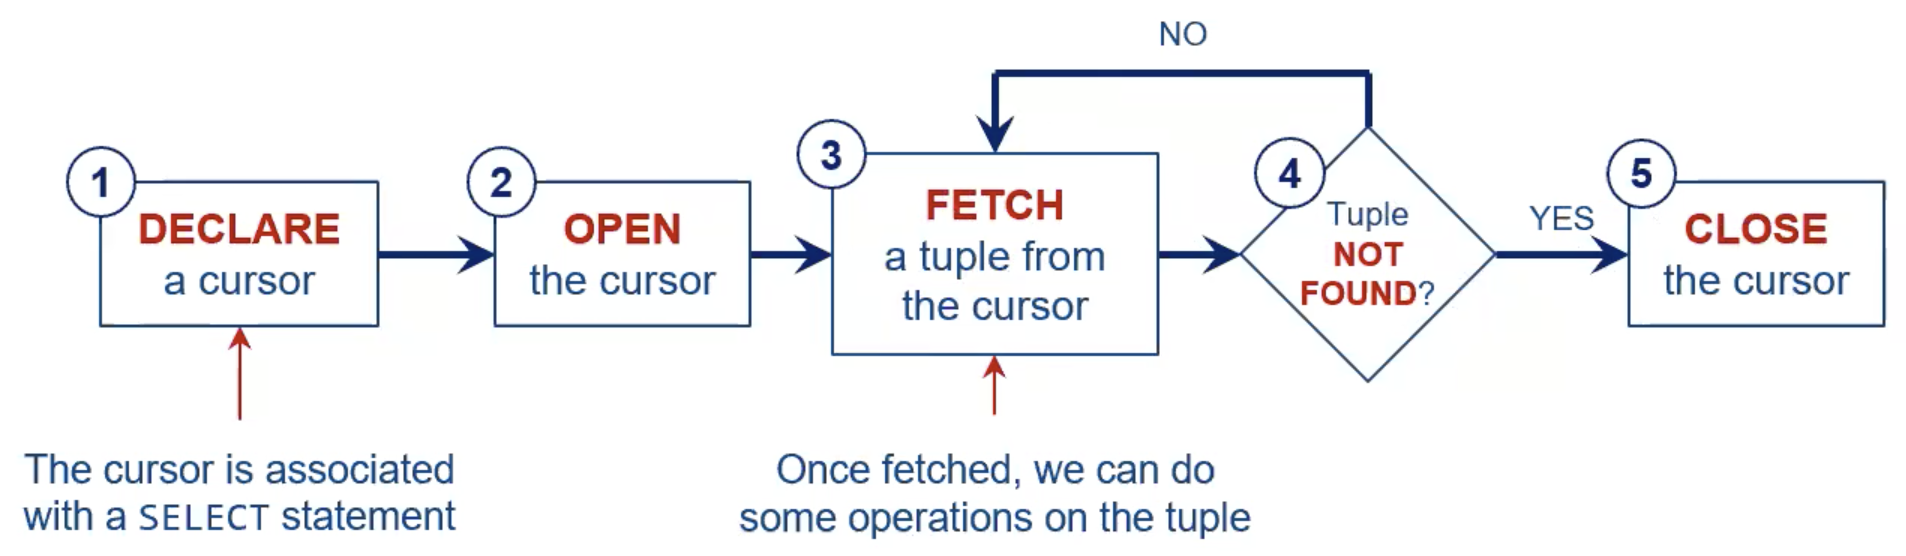
\includegraphics[width=0.9\linewidth]{cs2102-plpgsql-cursor.png} 
    \item e.g. Based on this ranking system of cryptocurrencies, I want to have daily record of first three coins from the TOP 10 cryptocurrencies that are down by more than 5\% in the past 7 days and are within 2 ranks apart from each other.
    \begin{lstlisting}[style=mySQL]
CREATE OR REPLACE FUNCTION consCryptosDown
(IN num INT)
RETURNS TABLE(rank INT, sym CHAR(4)) AS $$
DECLARE
  curs CURSOR FOR (SELECT * FROM cryptosRank
                   WHERE changes < -5);
  r1 RECORD;
  r2 RECORD;
BEGIN
  OPEN curs;
  LOOP 

  -- move cursor
  FETCH curs INTO r1;      /* loads tuples into r1 */
  EXIT WHEN NOT FOUND;     /* check for end of table */
  FETCH RELATIVE (num-1) FROM curs INTO r2;
  EXIT WHEN NOT FOUND;

  -- compare rows
  IF r2.rank - r1.rank = 2 THEN
    MOVE RELATIVE -(num) FROM curs;
      FOR c IN 1..num LOOP
      FETCH curs INTO r1;
      rank := r1.rank;
      sym := r1.symbol;
      RETURN NEXT;
    END LOOP;
    CLOSE curs;
    RETURN;
  END IF;

  MOVE RELATIVE -(num - 1) FROM curs;

  END LOOP;
  CLOSE curs;
END;
$$ LANGUAGE plpgsql;
    \end{lstlisting}
  \end{itemize}






\end{multicols}

\hrulefill \\
% \dotfill

\begin{multicols}{2}
  \section{SUMMARY: RELATIONAL MODEL}
  \begin{center}
    {\rowcolors{2}{gray!15}{gray!5}\begin{tabular}
        {ll}
        \rowcolor{cyan!10}
        \textbf{Term} & \textbf{Description} \\ \hline
        attribute & column of a table \\
        domain & set of possible values for an attribute \\
        attribute value & element of a domain \\ 
        relation schema & set of attributes (with their data types + relation name) \\
        relation & set of tuples \\
        tuple & roles of a table \\
        database schema & set of relation schemas \\
        database & set of relations / tables \\ 
        key & minimal set of attributes uniquely identifying a tuple in a relation \\
        primary key & selected key (in case of multiple candidate keys) \\
        foreign key & set of attributes that is a key in referenced relation \\
        prime attribute & attribute of a key \\
        \hline
      \end{tabular}
    }
  \end{center}

  \section{CONCEPTUAL EVALUATION OF QUERIES}
  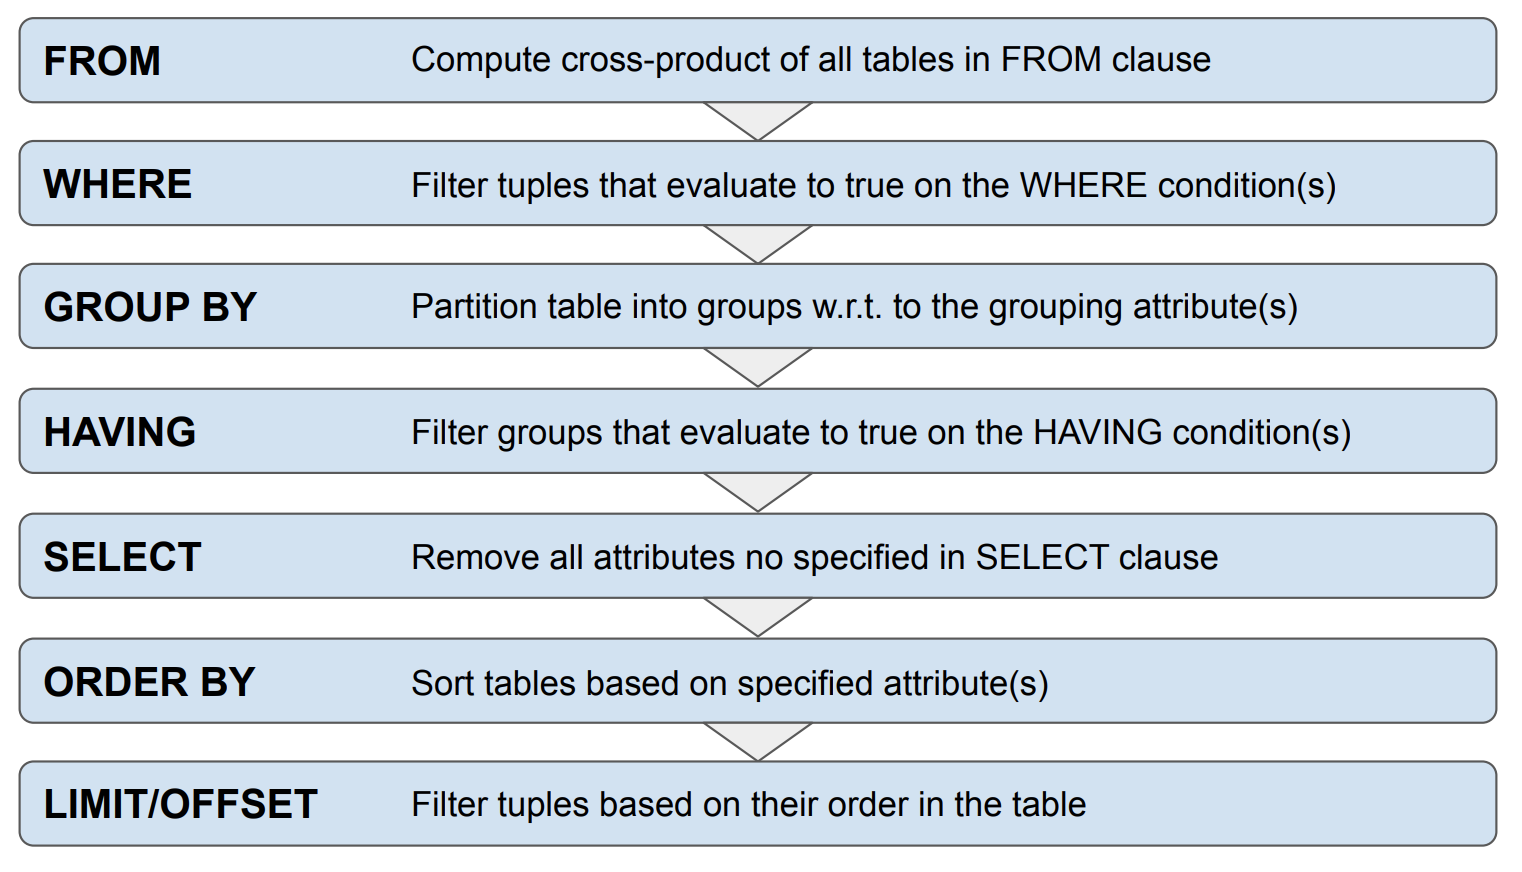
\includegraphics[width=0.9\linewidth]{cs2102-conceptual-evaluation-of-queries.png} 
\end{multicols}

\end{document}
